\documentclass[12pt,oneside]{memoir}
\usepackage[latinica]{matfmaster} 
\usepackage{svg}
\usepackage{array}
\usepackage{float}
\usepackage{tikz}
\usepackage{titlesec}
\usetikzlibrary{shapes, positioning}
\usepackage{amsmath}
\usepackage[ruled,vlined]{algorithm2e}
\usepackage{multirow}
\usepackage[table]{xcolor}

\maxtocdepth{subsection}
\maxsecnumdepth{subsection}

\bib{master}

\autor{Miloš Milaković}
\naslov{Sekvenciranje antibiotika - Elektronska lekcija}
\godina{2025}

\mentor{dr Jovana \textsc{Kovačević}, vanredni profesor\\ Univerzitet u Beogradu, Matematički fakultet}

\komisijaA{dr Mirjana \textsc{Maljković Ružičić}, docent\\ Univerzitet u Beogradu, Matematički fakultet}

\komisijaB{Nevena \textsc{Ćirić}, asistent\\ Univerzitet u Beogradu, Matematički fakultet}
% Datum odbrane (odkomentarisati narednu liniju i upisati datum odbrane ako je poznat)
% \datumodbrane{}

% Apstrakt na srpskom jeziku (u odabranom pismu)
\apstr{%
Ovaj rad predstavlja elektronsku lekciju posvećenu sekvenciranju antibiotika, sa fokusom na interaktivno upoznavanje sa različitim algoritamskim pristupima. Lekcija obuhvata teorijsko objašnjenje i vizuelizaciju sledećih algoritama za sekvenciranje proteina: gruba sila, \emph{Branch and Bound}, \emph{Leaderboard}, spektralna konvolucija i \emph{DeepNovo} sekvenciranje. Korisnicima je omogućeno da prate izvršavanje algoritama korak po korak, sa opcijama pauziranja i ponavljanja, čime se olakšava razumevanje kompleksnih procesa sekvenciranja. Ova interaktivna platforma može služiti kao edukativni alat za studente i predavače u oblasti bioinformatike.
}

% Ključne reči na srpskom jeziku (u odabranom pismu)
\kljucnereci{sekvenciranje, algoritmi, računarstvo, aminokiseline, maseni spektrometar, gruba sila, \emph{Branch and Bound}, \emph{Leaderboard}, \emph{DeepNovo}, spektralna konvolucija}

\begin{document}
\SetAlgorithmName{Algoritam}

% ==============================================================================
% Uvodni deo teze
\frontmatter
% ==============================================================================
\naslovna
\komisija
\posveta{Najvoljenijima}
\apstrakt
\tableofcontents*

% ==============================================================================
% Glavni deo teze
\mainmatter
% ==============================================================================

% ------------------------------------------------------------------------------
\chapter{Uvod}
% ------------------------------------------------------------------------------
Sekvenciranje bioloških molekula predstavlja proces određivanja preciznog redosleda gradivnih jedinica od kojih su sastavljeni. Tako, na primer, govorimo o sekvenciranju DNK, kojim se utvrđuje niz nukleotida u genomu organizma. Međutim, osim genoma, moguće je sekvencirati i proteine, pri čemu se određuje redosled aminokiselina koji čini njihovu primarnu strukturu. Takav postupak naziva se sekvenciranje proteina.

Iako se sekvenciranje genoma i sekvenciranje proteina oslanja na eksperimentalne tehnike, genom se, zahvaljujući univerzalnom genetskom kodu, može relativno jednostavno odrediti, dok se struktura proteina ne može direktno predvideti iz genetske informacije i zahteva dodatne metode, poput masene spektrometrije. U prirodi postoji 20 standardnih aminokiselina (slika \ref{fig:aminokiseline}) koje se kombinuju u različitim sekvencama kako bi formirale proteine. U kontekstu antibiotika, specifičan redosled aminokiselina je od presudnog značaja jer direktno utiče na:

\begin{itemize}
    \item Trodimenzionalnu strukturu molekula
    \item Biološku aktivnost i mehanizam dejstva
\end{itemize}

Mnogi savremeni antibiotici predstavljaju peptide, što znači da su zapravo kratki lanci aminokiselina, tj. mali proteini. Antibiotici predstavljaju hemijska jedinjenja koja uništavaju mikroorganizme ili inhibiraju njihov rast, čime imaju ključnu ulogu u borbi protiv infekcija. Zbog njihove biološke važnosti i sve izraženijeg problema antimikrobne rezistencije, sekvenciranje antibiotika predstavlja značajnu oblast istraživanja u savremenoj bioinformatici i farmaceutskoj industriji. Zbog toga, ovaj rad će se fokusirati upravo na proces sekvenciranja antibiotika.

\begin{figure}[h]
  \centering
  \includesvg[width=0.8\textwidth]{images/amino-acids-table.svg}
  \caption{Esencijalne aminokiseline sa svojim masama izraženim u daltonima (Da)}
  \label{fig:aminokiseline}
\end{figure}

\section{Cilj rada}
U ovom radu implementirana je interaktivna elektronska platforma namenjena prikazu algoritamskih pristupa za sekvenciranje antibiotika, sa fokusom na njihovu vizuelizaciju u realnom vremenu. Platforma korisnicima omogućava da se istraže principi i rad savremenih algoritama kroz interaktivne simulacije, čime se olakšava razumevanje kompleksnih bioinformatičkih koncepata.

Glavni ciljevi ovog rada su:
\begin{itemize}
    \item Pružiti pregled modernih algoritama za sekvenciranje antibiotika
    \item Razviti interaktivnu edukativnu platformu za vizuelizaciju sekvenciranja
\end{itemize}

Rad je posebno koristan studentima bioinformatike i molekularne biologije kao alat za bolje razumevanje algoritama za rekonstrukciju peptidnih sekvenci.

% ------------------------------------------------------------------------------
\chapter{Teorijske osnove}
% ------------------------------------------------------------------------------

\section{Centralna dogma molekularne biologije}
Proces sekvenciranja antibiotika je fundamentalan u razumevanju kako su ovi molekuli proizvedeni od strane bakterija i kako se oni mogu sintetisati ili modifikovati za primene u medicini. Antibiotici su često peptidi, pri čemu veliki broj pripada neribozomalnim peptidima (\emph{non-ribosomal peptides - NRPs}), koji ne prate standardna pravila za sintezu proteina čime se otežava njihovo sekvenciranje \cite{online_lecture, online_book}.

DNK sadrži recept za kreiranje proteina. Naime, DNK se sastoji od gena koji mogu biti uključeni i tada će se na osnovu njih kreirati proteini ili isključeni kada se oni neće koristiti za kreiranje proteina. Ovaj proces uključivanja i isključivanja gena naziva se genska ekspresija i zavisi od toga da li je potrebno da se određeni protein kreira ili ne (na primer, fotosinteza kod biljaka koja se obavlja samo preko dana).
Najveći broj proteina nastaje kroz proces koji se zove centralna dogma molekularne biologije, koja kaže da se DNK prvo prepisuje u RNK (slika \ref{fig:transkripcija}), a zatim se RNK prevodi u protein. Proces prevođenja DNK u RNK naziva se transkripcija i on podrazumeva da enzim RNK polimeraza očitava jedan lanac DNK i na osnovu njega sintetiše jedan, komplementaran RNK lanac, pri čemu se nukleotid timin (T) zamenjuje uracilom (U). Na slici \ref{fig:transkripcija} se može se primetiti da se DNK sastoji od 2 lanca koja su komplementarna. Enzim RNK polimeraza se zakači na DNK lanac ka početku gena, zatim se kreće duž gena čime razdvaja dva lanca DNK i tako stvara prostor za prepisivanje DNK čime se dobija novi molekul RNK.

\begin{figure}[h]
  \centering
  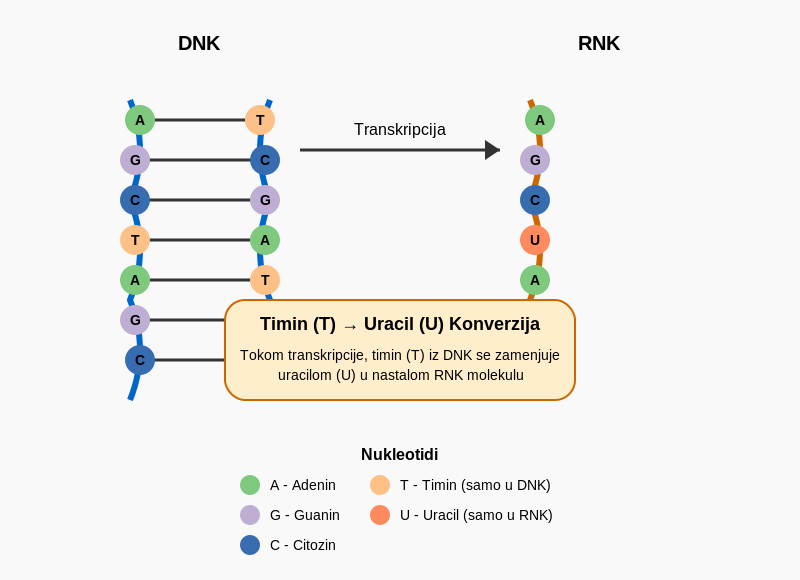
\includegraphics[width=0.8\textwidth]{images/dna_rna_transcription_diagram.png}
  \caption{Transkripcija DNK u RNK}
  \label{fig:transkripcija}
\end{figure}

Prilikom prevođenja RNK u protein potrebno je na osnovu nukleotida odrediti koja je aminokiselina u pitanju. Za ovaj proces je zadužena organela ribozom, koja omogućava očitavanje informacija koju nosi RNK prema unapred utvrđenom pravilu koje se naziva genetski kod. Budući da je potrebno uniformno tumačiti nukleotidnu sekvencu, koristi se niz od tri uzastopna nukleotida, poznat kao kodon. Upotrebom kodona dužine tri nukleotida dobija se ukupno 64 različite sekvence, koje se mapiraju na 20 različitih aminokiselina. Da je korišćen niz od samo dva nukleotida, bilo bi moguće formirati svega 16 kombinacija, što ne bi bilo dovoljno da se pokriju sve aminokiseline neophodne za sintezu proteina. Na slici \ref{fig:codon-wheel} može se videti kako se kodoni prevode u odgovarajuće aminokiseline. Postoje start i stop kodoni koji određuju početak odnosno kraj sekvence koja se prevodi u protein.

\begin{figure}[H]
  \centering
  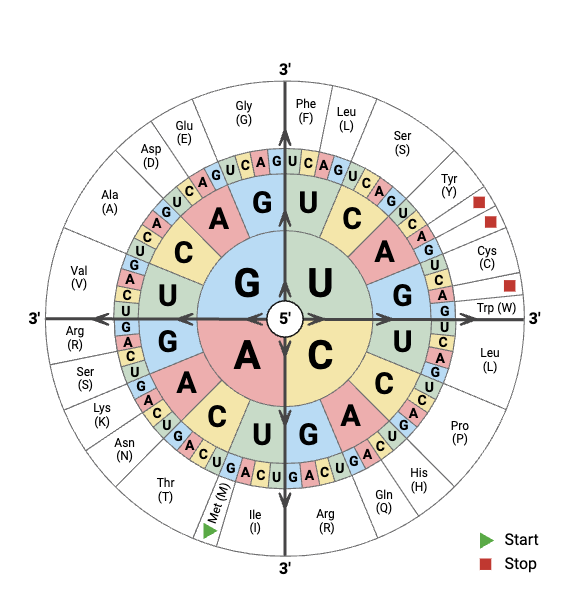
\includegraphics[width=0.8\textwidth]{images/RNA-Codon-Wheel.png}
  \caption{RNK kodonski točak prikazuje kako se sekvence od tri nukleotida (kodoni) prevode u aminokiseline. Svaki kodon se čita od centra ka spolja, a zeleni trougao označava start kodon (AUG) koji kodira metionin, dok crveni kvadrati označavaju stop kodone (UAA, UAG, UGA) koji određuju kraj sekvence koja se prevodi u protein. Preuzeto sa \cite{codon_chart}.}
  \label{fig:codon-wheel}
\end{figure}


\section{Odstupanje od centralne dogme}
Tirocidin B1 je cikličan peptid dužine 10 (slika \ref{fig:tirocidin}), što znači da su prva i poslednja aminokiselina povezane i da samim tim postoji 10 njegovih različitih linearnih reprezentacija (tabela \ref{tab:linear_representations}). Prateći centralnu dogmu i činjenicu da se 1 kodon prevodi u 1 aminokiselinu, bilo je za očekivati da je moguće pronaći 10 kodona odnosno 30 nukleotida u genomu bakterije \emph{Bacillus brevis} od koje nastaje ovaj antibiotik. Da bi se ovaj postupak obavio, potrebno je proveriti više hiljada 30-grama koji mogu da počnu bilo gde u genomu, što može delovati kao dugotrajan zadatak, ali uz moderne računare je ostvariv u prihvatljivom vremenu. Analiziranjem genoma utvrđeno je da ne postoji 30-gram koji se kodira u neki od 10 različitih reprenzatacija traženog antibiotika.

\begin{table}[h]
\centering
\begin{tabular}{ll}
\toprule
\# & Linearna sekvenca \\
\midrule
1 & \textcolor{red}{Lys} – \textcolor{blue}{Leu} – \textcolor{orange}{Phe} – \textcolor{violet}{Pro} – \textcolor{teal}{Trp} – \textcolor{orange}{Phe} – \textcolor{magenta}{Asn} – \textcolor{brown}{Gln} – \textcolor{cyan}{Tyr} – \textcolor{green!70!black}{Val} \\
2 & \textcolor{blue}{Leu} – \textcolor{orange}{Phe} – \textcolor{violet}{Pro} – \textcolor{teal}{Trp} – \textcolor{orange}{Phe} – \textcolor{magenta}{Asn} – \textcolor{brown}{Gln} – \textcolor{cyan}{Tyr} – \textcolor{green!70!black}{Val} – \textcolor{red}{Lys} \\
3 & \textcolor{orange}{Phe} – \textcolor{violet}{Pro} – \textcolor{teal}{Trp} – \textcolor{orange}{Phe} – \textcolor{magenta}{Asn} – \textcolor{brown}{Gln} – \textcolor{cyan}{Tyr} – \textcolor{green!70!black}{Val} – \textcolor{red}{Lys} – \textcolor{blue}{Leu} \\
4 & \textcolor{violet}{Pro} – \textcolor{teal}{Trp} – \textcolor{orange}{Phe} – \textcolor{magenta}{Asn} – \textcolor{brown}{Gln} – \textcolor{cyan}{Tyr} – \textcolor{green!70!black}{Val} – \textcolor{red}{Lys} – \textcolor{blue}{Leu} – \textcolor{orange}{Phe} \\
5 & \textcolor{teal}{Trp} – \textcolor{orange}{Phe} – \textcolor{magenta}{Asn} – \textcolor{brown}{Gln} – \textcolor{cyan}{Tyr} – \textcolor{green!70!black}{Val} – \textcolor{red}{Lys} – \textcolor{blue}{Leu} – \textcolor{orange}{Phe} – \textcolor{violet}{Pro} \\
6 & \textcolor{orange}{Phe} – \textcolor{magenta}{Asn} – \textcolor{brown}{Gln} – \textcolor{cyan}{Tyr} – \textcolor{green!70!black}{Val} – \textcolor{red}{Lys} – \textcolor{blue}{Leu} – \textcolor{orange}{Phe} – \textcolor{violet}{Pro} – \textcolor{teal}{Trp} \\
7 & \textcolor{magenta}{Asn} – \textcolor{brown}{Gln} – \textcolor{cyan}{Tyr} – \textcolor{green!70!black}{Val} – \textcolor{red}{Lys} – \textcolor{blue}{Leu} – \textcolor{orange}{Phe} – \textcolor{violet}{Pro} – \textcolor{teal}{Trp} – \textcolor{orange}{Phe} \\
8 & \textcolor{brown}{Gln} – \textcolor{cyan}{Tyr} – \textcolor{green!70!black}{Val} – \textcolor{red}{Lys} – \textcolor{blue}{Leu} – \textcolor{orange}{Phe} – \textcolor{violet}{Pro} – \textcolor{teal}{Trp} – \textcolor{orange}{Phe} – \textcolor{magenta}{Asn} \\
9 & \textcolor{cyan}{Tyr} – \textcolor{green!70!black}{Val} – \textcolor{red}{Lys} – \textcolor{blue}{Leu} – \textcolor{orange}{Phe} – \textcolor{violet}{Pro} – \textcolor{teal}{Trp} – \textcolor{orange}{Phe} – \textcolor{magenta}{Asn} – \textcolor{brown}{Gln} \\
10 & \textcolor{green!70!black}{Val} – \textcolor{red}{Lys} – \textcolor{blue}{Leu} – \textcolor{orange}{Phe} – \textcolor{violet}{Pro} – \textcolor{teal}{Trp} – \textcolor{orange}{Phe} – \textcolor{magenta}{Asn} – \textcolor{brown}{Gln} – \textcolor{cyan}{Tyr} \\
\bottomrule
\end{tabular}
\caption{Deset različitih linearnih reprezentacija tirocidina B1}
\label{tab:linear_representations}
\end{table}

\begin{figure}[h]
  \centering
  \includesvg[width=0.8\textwidth]{images/tyrocidine.svg}
  \caption{Struktura tirocidina B1, cikličnog peptida sastavljenog od 10 aminokiselina.}
  \label{fig:tirocidin}
\end{figure}

Na ovaj način je pokazano da Tirocidin B1 ne prati centralnu dogmu molekularne biologije i da ovaj peptid nastaje kroz drugačiji proces, uz pomoć posebnih enzima koji su zaduženi za njihovo sintentisanje. Oni se zovu \emph{NRP} sintetaze. Ovi enzimi se sastoje od kompleksnih molekulskih jedinica, takozvanih modula, gde svaki modul odgovara jednoj aminokiselini koja učestvuje u sastavu proteina. U slučaju Tirocidina B1, enzim sadrži 10 modula i svaki od modula kodira 1 aminokiselinu čime je određena struktura antibiotika.

Samim tim, pošto struktura proteina nije određena na osnovu genoma bakterije, metode za sekvencioniranje DNK ovde nisu od pomoći i potrebno je sekvencirati direktno sam peptid.

\section{Maseni spektrometar}
Maseni spektrometar je mašina za merenje masa molekula, uključujući mase peptida i proteina. Alat funkcioniše na principu analize više uzoraka istog peptida, tako što date uzorke deli na sve moguće potpeptide, nakon čega se određuju mase potpeptida. U realnosti uzorak se pretvara u naelektrisane jone da bi na njih mogli da utiču električno i magnetno polje. Potom se joni dele na osnovu odnosa mase i naelektrisanja, a njihove vrednosti se zatim precizno mere \cite{spectrometer}.

Masa se meri u daltonima (Da), pri čemu je 1 Da približno jednak masi protona/neutrona. Samim tim masa molekula je jednaka sumi masa protona/neutrona koji čine taj molekul. Mase aminokiselina su poznate i prikazane su na Slici \ref{fig:aminokiseline}. Može se primetiti da neke aminokiseline imaju istu masu, tako da 20 različitih aminokiselina ima 18 različitih masa.

Samim tim na osnovu poznatih masa aminokiselina možemo da odredimo masu celog peptida. Na primer, masa tirocidina se može izračunati na sledeći način:
\begin{verbatim}
 V    K     L     F     P    W     F     N     Q     Y     
99 + 128 + 113 + 147 + 97 + 186 + 147 + 114 + 128 + 163 = 1322
\end{verbatim}

\section{Teorijski spektar peptida}
Teorijski spektar peptida predstavlja mase svih mogućih potpeptida, uključujući 0 i masu celog peptida. Na osnovu peptida možemo lako da odredimo teorijski spektar ali na osnovu spektra ne možemo lako da odredimo koji je peptid u pitanju.

Problem sekvenciranja ciklopeptida samim tim se svodi na problem kako rekonstruisati ciklični peptid na osnovu njegovog teorijskog spektra. U nastavku će biti prikazano nekoliko različitih algoritama za sekvenciranje peptida.

Kao ulaz u svaki od ovih algoritama očekuje se eksperimentalni spektar, odnosno spektar koji je dobijen uz pomoć masenog spektrometra za neki peptid. Na slici \ref{fig:spektar} su prikazane mase svih potpeptida peptida \textbf{NQEL} koje se dobijaju uz pomoć masenog spektrometra, kao i masa praznog peptida i celog peptida, takođe je prikazan i teorijski spektar.

\begin{figure}[h]
  \centering
  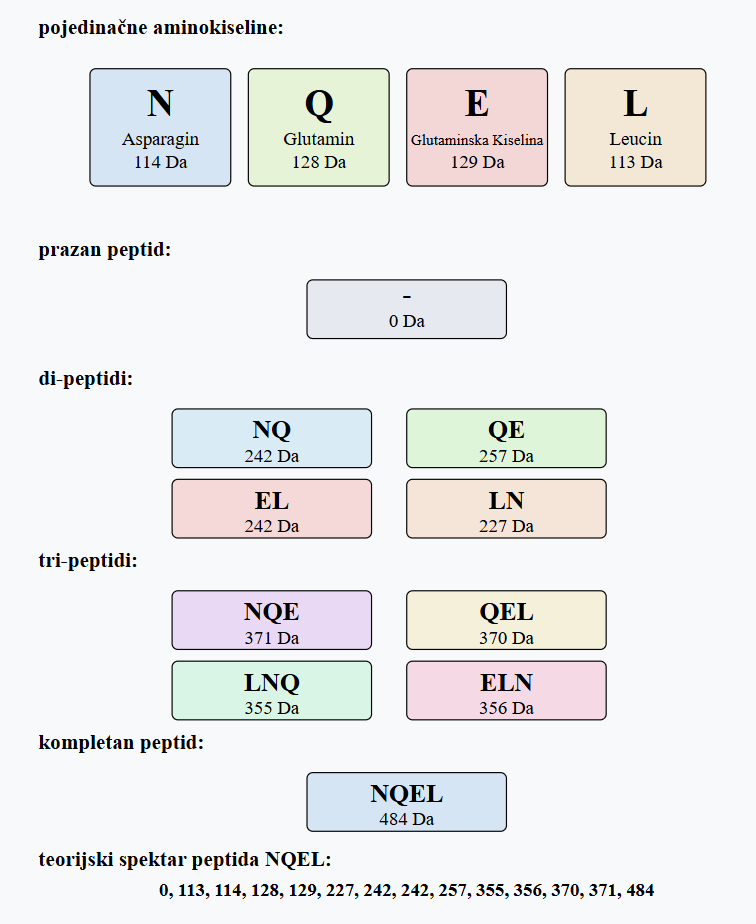
\includegraphics[width=0.9\textwidth]{images/peptide-theoretical-spectrum.png}
  \caption{Teorijski spektar peptida \textbf{NQEL} koji prikazuje sve moguće potpeptide, njihove mase i njegov teorijski spektar}
  \label{fig:spektar}
\end{figure}


% ------------------------------------------------------------------------------
\chapter{Algoritmi za sekvenciranje}
% ------------------------------------------------------------------------------
U ovom odeljku biće prikazani algoritmi za određivanje cikličnog peptida na osnovu poznatog eksperimentalnog spektra. Neki od algoritama koji će biti objašnjeni su:
\begin{itemize}
    \item \textbf{Algoritam grube sile} (\emph{Brute force}): Direktan pristup gde se isprobavaju sve moguće kombinacije da bi se našlo optimalno rešenje.
    \item \textbf{\emph{Branch and Bound}}: Optimizovan algoritam koji će odbacivati kandidate čim prestanu da budu potencijalno rešenje.
    \item \textbf{\emph{Leaderboard} algoritam}: Algoritam koji održava listu \emph{N} najboljih kandidata za rešenje i na osnovu njih smanjuje broj potencijalnih kandidata.
    \item \textbf{Spektralna konvolucija}: Određuje aminokiseline koje mogu da učestvuju u peptidu na osnovu eksperimentalnog spektra.
    \item \textbf{\emph{DeepNovo}}: Metoda zasnovana na dubokom učenju koja omogućava sekvenciranje peptida bez oslanjanja na baze podataka.
\end{itemize}

\section{Gruba sila (\emph{Brute Force})}
Najosnovniji pristup sekvenciranju koji sistematski ispituje sve moguće kombinacije aminokiselina dok ne pronađe sekvencu koja najbolje odgovara eksperimentalnom spektru \cite{online_lecture, online_book}. Iako jednostavan za implementaciju, ovaj pristup postaje neizvodiv za duže sekvence zbog eksponencijalnog rasta prostora pretrage.

Na primer, za peptid mase 579 Da, algoritam će generisati sve moguće kombinacije aminokiselina i proveriti da li njihova ukupna masa odgovara zadatoj masi. Kao što je prikazano u tabeli \ref{tab:primer1}, mogu postojati različiti peptidi sa istom ukupnom masom (\textbf{FPAYT} i \textbf{QNWGS}), što dodatno komplikuje problem.

\begin{table}[h]
\centering
\begin{tabular}{>{\centering\arraybackslash}m{1cm} r @{\hskip 1cm} >{\centering\arraybackslash}m{1cm} r}
\toprule
\textbf{F} & 147 Da & \textbf{Q} & 128 Da \\
\textbf{P} & 97 Da  & \textbf{N} & 114 Da \\
\textbf{A} & 71 Da  & \textbf{W} & 186 Da \\
\textbf{Y} & 163 Da & \textbf{G} & 57 Da  \\
\textbf{T} & 101 Da & \textbf{S} & 94 Da  \\
\midrule
\multicolumn{2}{r}{\textbf{Ukupna masa:} 579 Da} &
\multicolumn{2}{r}{\textbf{Ukupna masa:} 579 Da} \\
\bottomrule
\end{tabular}
\caption{Poređenje aminokiselina i njihove mase}
\label{tab:primer1}
\end{table}

Da bi se utvrdilo koji od peptida je tačno rešenje, algoritam mora da generiše teorijski spektar za svaki kandidat peptid i uporedi ga sa eksperimentalnim spektrom. Ovo dodatno povećava računsku složenost algoritma, ali je neophodno za pronalaženje tačnog rešenja.

Na slici \ref{fig:same_mass}, možemo da vidimo koliko postoji različitih peptida za istu masu, samim tim možemo zaključiti da je izvršavanje algoritma grube sile veoma neefikasno.

\begin{figure}[h]
  \centering
  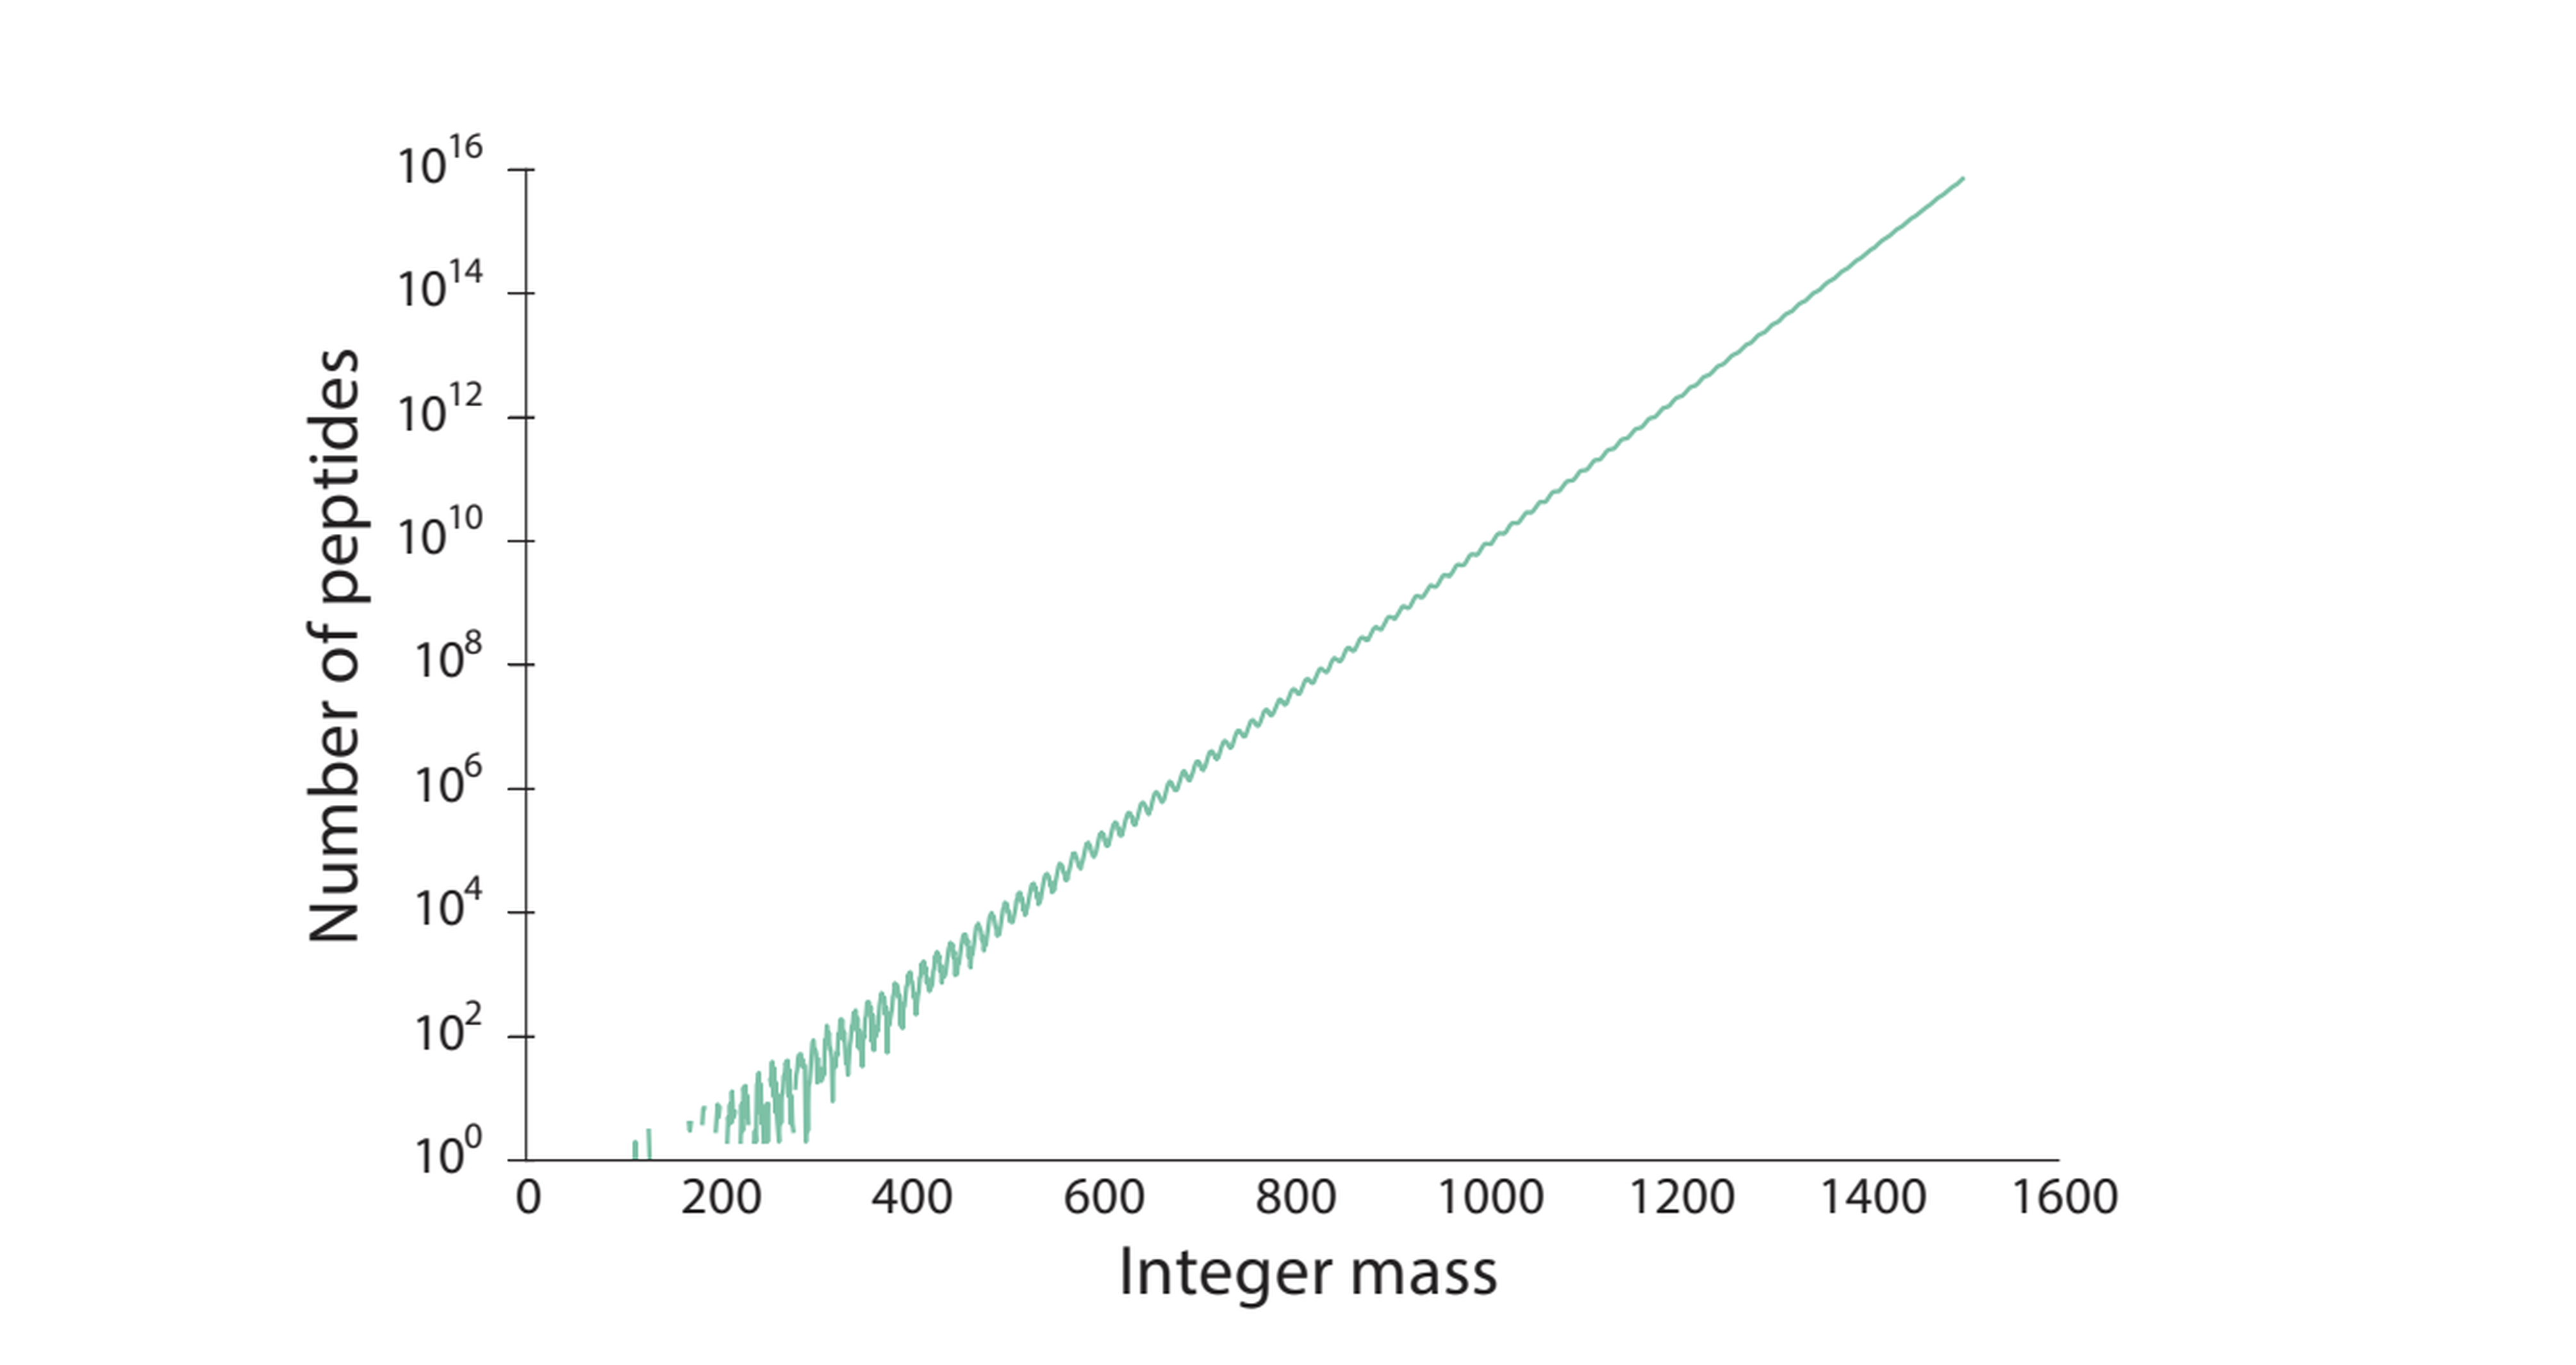
\includegraphics[width=0.9\textwidth]{images/number_of_peptides_with_same_mass.png}
  \caption{Broj peptida koji imaju istu masu. Preuzeto iz \cite{online_book}.}
  \label{fig:same_mass}
\end{figure}

Na osnovu prethodnog teksta definiše se pseudokod za algoritam grube sile koji se može videti kao algoritam \ref{alg:brute_force}.

\begin{algorithm}[H]
\label{alg:brute_force}
\caption{Gruba sila}
\SetAlgoLined
\DontPrintSemicolon
\SetKwFunction{FRec}{GrubaSila}
\SetKwProg{Fn}{Funkcija}{}{}
\Fn{\FRec{eksperimentalniSpektar}}{
    $peptidi \gets$ Lista sa praznim stringom\;
    $rezultati \gets$ Prazna lista\;
    $ciljna\_masa \gets$ Poslednji element $eksperimentalniSpektar$\;
    
    \While{$peptidi \neq$ Prazno}{
        $prosireni \gets$ \textbf{Proširi}($peptidi$)\;
        $kandidati \gets$ Prazna lista\;
    
        \ForEach{$peptid \in prosireni$}{
            $masa \gets$ \textbf{IzračunajMasu}($peptid$)\;
    
            \uIf{$masa = ciljna\_masa$}{
                \If{\textbf{CikličniSpektar}($peptid$) $=$ $eksperimentalniSpektar$}{
                    Dodaj $peptid$ u $rezultati$\;
                }
            }\ElseIf{$masa < ciljna\_masa$}{
                Dodaj $peptid$ u $kandidati$\;
            }
        }
    
        $peptidi \gets kandidati$\;
    }
    
    \Return{$rezultati$}\;
}
\end{algorithm}

\noindent
\textbf{Objašnjenje pomoćnih funkcija:}
\begin{itemize}
  \item \textbf{Proširi(peptidi)} – sve preostale peptide proširuje sa svakom mogućom aminokiselinom i vraća proširenu listu.
  \item \textbf{IzračunajMasu(peptid)} – računa ukupnu masu peptida sabiranjem masa svih aminokiselina koje čine taj peptid.
  \item \textbf{CikličniSpektar(peptid)} – za peptid koji je potencijalno rešenje generiše se ciklični spektar koji se poredi sa zadatim eksperimentalnim spektrom.
\end{itemize}

\section{\emph{Branch and Bound}}
\emph{Branch and Bound} algoritam \cite{online_lecture, online_book} je optimizovana verzija algoritma grube sile koja koristi strategiju „podeli pa vladaj“ za efikasnije pretraživanje prostora rešenja. Za razliku od algoritma grube sile koji ispituje sve moguće kombinacije, \emph{Branch and Bound} algoritam inteligentno eliminiše delove prostora pretrage koji ne mogu sadržati optimalno rešenje.

U kontekstu sekvenciranja peptida, algoritam funkcioniše na sledeći način:
\begin{itemize}
    \item \textbf{Grananje (\emph{Branch}):} Algoritam gradi stablo pretrage gde svaki čvor predstavlja delimičnu sekvencu peptida. Svaki čvor se grana dodavanjem nove aminokiseline na postojeću sekvencu.
    \item \textbf{Ograničavanje (\emph{Bound}):} Za svaki čvor, algoritam procenjuje da li taj put može dovesti do validnog rešenja. Ako masa peptida već premašuje ciljanu masu ili ako teorijski spektar delimične sekvence nije u skladu sa eksperimentalnim, ta grana se odseca i dalje se ne istražuje.
    \item \textbf{Optimizacija:} Algoritam može koristiti dodatne heuristike za procenu koje grane prvo istražiti, što dodatno ubrzava pronalaženje rešenja.
\end{itemize}

Prednosti \emph{Branch and Bound} algoritma u odnosu na algoritam grube sile su značajne i njihovo poređenje može da se vidi u tabeli \ref{tab:branch_vs_brute}.

\begin{table}[H]
\centering
\renewcommand{\arraystretch}{1.5}
\begin{tabular}{|>{\raggedright\arraybackslash}m{0.45\textwidth}|>{\raggedright\arraybackslash}m{0.45\textwidth}|}
\hline
\textbf{Algoritam grube sile} & \textbf{Branch and Bound} \\
\hline
Istražuje sve moguće kombinacije & Inteligentno eliminiše neperspektivne grane \\
\hline
Eksponencijalna vremenska složenost & Značajno bolja vremenska složenost (u najgorem slučaju i dalje eksponencijalna, ali znatno brža) \\
\hline
Garantuje pronalaženje svih rešenja & I dalje garantuje pronalaženje svih rešenja \\
\hline
Neefikasan za duže peptide & Efikasniji za duže peptide \\
\hline
\end{tabular}
\caption{Poređenje algoritma grube sile i Branch and Bound pristupa}
\label{tab:branch_vs_brute}
\end{table}

Pseudokod za algoritam Branch and Bound može se videti kao algoritam \ref{alg:branch_and_bound}.

\begin{algorithm}[H]
\label{alg:branch_and_bound}
\caption{Branch and Bound}
\SetAlgoLined
\DontPrintSemicolon
\SetKwFunction{FRec}{BranchAndBound}
\SetKwProg{Fn}{Funkcija}{}{}
\Fn{\FRec{eksperimentalniSpektar}}{
    $peptidi \gets$ Lista sa praznim stringom\;
    $rezultati \gets$ Prazna lista\;
    $ciljna\_masa \gets$ Poslednji element $eksperimentalniSpektar$\;
    
    \While{$peptidi \neq$ Prazno}{
        $prosireni \gets$ \textbf{Proširi}($peptidi$)\;
        $kandidati \gets$ Prazna lista\;
    
        \ForEach{$peptid \in prosireni$}{
            $masa \gets$ \textbf{IzračunajMasu}($peptid$)\;

            \uIf{$masa = ciljna\_masa$}{
                \If{\textbf{CikličniSpektar}($peptid$) $=$ $eksperimentalniSpektar$}{
                    Dodaj $peptid$ u $rezultati$\;
                }
            }\ElseIf{$masa < ciljna\_masa$}{
                \If{\textbf{Konzistentan}($peptid$, $eksperimentalniSpektar$)}{
                    Dodaj $peptid$ u $kandidati$\;
                }
            }

        }
    
        $peptidi \gets kandidati$\;
    }
    
    \Return{$rezultati$}\;
}
\end{algorithm}

\noindent
\textbf{Objašnjenje pomoćnih funkcija:}
\begin{itemize}
  \item \textbf{Konzistentan(peptid, eksperimentalniSpektar)} – glavni korak odsecanja i smanjivanja prostora pretrage.  Provera da li se svaka masa u okviru linearnog spektra peptida javlja i u okviru eksperimentalnog spektra. Ako neka masa postoji u okviru linearnog spektra a ne u okviru eksperimentalnog spektra to znaci da spektrum nije konzistentan, obrnuto ne mora da važi, jer se računa spektar parcijalnog peptida a ne još celog pa masa koja trenutno nije prisutna može da se pojavi.
\end{itemize}

\section{Uporedna analiza prethodnih algoritama}

Posmatramo primer sa 3 aminokiseline:
\begin{itemize}
    \item A (masa = 100 Da)
    \item B (masa = 150 Da)
    \item C (masa = 200 Da)
\end{itemize}

Tražimo sekvencu AB (ukupna masa = 250 Da). Poredimo algoritme grube sile i grananja i ograničavanja.

\subsection{Algoritam grube sile}
Ispituje sve kombinacije i odbacuje samo kada ukupna masa premaši traženu masu:

\begin{center}
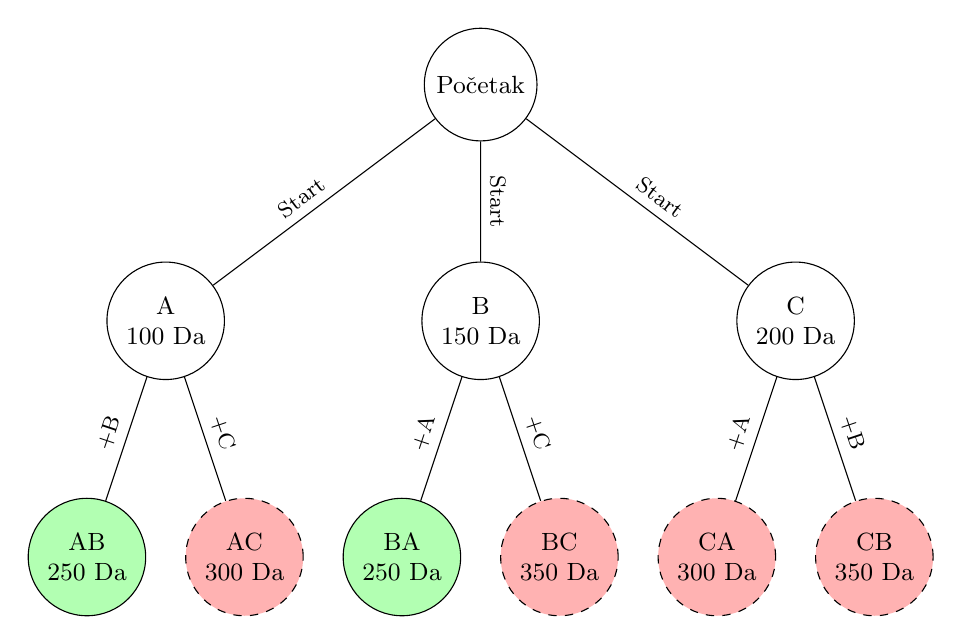
\begin{tikzpicture}[
    level distance=3cm,
    level 1/.style={sibling distance=4cm},
    level 2/.style={sibling distance=2cm},
    node/.style={draw, circle, minimum size=1.2cm, font=\small, align=center},
    solution/.style={fill=green!30},
    pruned/.style={fill=red!30, dashed},
    edge label/.style={font=\footnotesize, midway, sloped}]

% Root node
\node[node] (root) {Početak}
% First level - single amino acids
    child {
        node[node] (a) {A \\ 100 Da}
        % Second level - pairs
        child {
            node[node, solution] (ab) {AB \\ 250 Da}
            edge from parent node[edge label, above] {+B}
        }
        child {
            node[node, pruned] (ac) {AC \\ 300 Da}
            edge from parent node[edge label, above] {+C}
        }
        edge from parent node[edge label, left=0.2cm, above] {Start}
    }
    child {
        node[node] (b) {B \\ 150 Da}
        child {
            node[node, solution] (ba) {BA \\ 250 Da}
            edge from parent node[edge label, above] {+A}
        }
        child {
            node[node, pruned] (bc) {BC \\ 350 Da}
            edge from parent node[edge label, above] {+C}
        }
        edge from parent node[edge label, above] {Start}
    }
    child {
        node[node] (c) {C \\ 200 Da}
        child {
            node[node, pruned] (ca) {CA \\ 300 Da}
            edge from parent node[edge label, above] {+A}
        }
        child {
            node[node, pruned] (cb) {CB \\ 350 Da}
            edge from parent node[edge label, above] {+B}
        }
        edge from parent node[edge label, right=0.2cm, above] {Start}
    };

% Add vertical space manually
\node[below=0.5cm of a] (dummy-a) {};
\node[below=0.5cm of b] (dummy-b) {};
\node[below=0.5cm of c] (dummy-c) {};

\end{tikzpicture}
\end{center}

\textbf{Objašnjenje:}
\begin{itemize}
    \item \textcolor{green!50!black}{Zeleno} - pronađena rešenja (AB, BA)
    \item \textcolor{red!50!black}{Crveno} - odbačene grane (masa > 250 Da)
    \item Ukupno evaluacija: 3 (prvi nivo) + 6 (drugi nivo) = 9 čvorova
\end{itemize}

\subsection{Algoritam \emph{Branch and Bound}}
Odbacuje grane gde bilo koji deo sekvence nema masu koja postoji u eksperimentalnom spektru:

\begin{center}
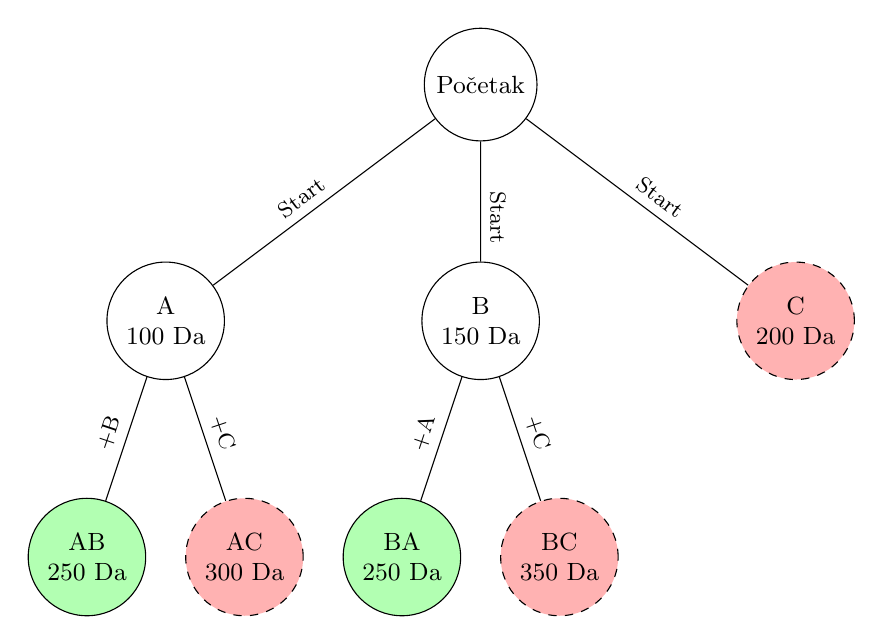
\begin{tikzpicture}[
    level distance=3cm,
    level 1/.style={sibling distance=4cm},
    level 2/.style={sibling distance=2cm},
    node/.style={draw, circle, minimum size=1.2cm, font=\small, align=center},
    solution/.style={fill=green!30},
    pruned/.style={fill=red!30, dashed},
    edge label/.style={font=\footnotesize, midway, sloped}]

% Root node
\node[node] {Početak}
% First level
    child {
        node[node] (a) {A \\ 100 Da}
        % Second level - pairs
        child {
            node[node, solution] (ab) {AB \\ 250 Da}
            edge from parent node[edge label, above] {+B}
        }
        child {
            node[node, pruned] (ac) {AC \\ 300 Da}
            edge from parent node[edge label, above] {+C}
        }
        edge from parent node[edge label, left=0.2cm, above] {Start}
    }
    child {
        node[node] {B \\ 150 Da}
        child {
            node[node, solution] (ba) {BA \\ 250 Da}
            edge from parent node[edge label, above] {+A}
        }
        child {
            node[node, pruned] (bc) {BC \\ 350 Da}
            edge from parent node[edge label, above] {+C}
        }
        edge from parent node[edge label, right=0.2cm, above] {Start}
    }
    child {
        node[node, pruned] {C \\ 200 Da}
        edge from parent node[edge label, right=0.2cm, above] {Start}
    };

\end{tikzpicture}
\end{center}

\textbf{Objašnjenje:}
\begin{itemize}
    \item \textcolor{green!50!black}{Zeleno} - pronađena rešenja (AB, BA)
    \item \textcolor{red!50!black}{Crveno} - odbačene grane (C nema masu iz spektra)
    \item Ukupno evaluacija: 3 (prvi nivo) + 4 (drugi nivo) = 7 čvorova
\end{itemize}

\subsection{Zaključak}

Algoritam grananja i ograničavanja značajno smanjuje prostor pretrage eliminacijom neperspektivnih grana već u ranim fazama, dok gruba sila mora da ispita sve kombinacije.
Na ovom primeru može se primetiti kako se odmah odbacuje cela \textbf{C} grana i svi njeni potomci. U ovom slučaju smanjuje se prostor pretrage za samo dva čvora, ali u stvarnosti postoji 20 aminokiselina i odsecanje čvorova i njihovih potomaka u samom startu predstavlja ogromno ubrzanje i poboljšanje u odnosu na algoritam grube sile.

\section{\emph{Leaderboard} algoritam}
\emph{Leaderboard} algoritam \cite{online_lecture, online_book} predstavlja optimizovani pristup za sekvenciranje peptida. Za razliku od sekvenciranja grubom silom koje zahteva tačno poklapanje između teorijskog spektra kandidata i eksperimentalnog spektra, ovaj algoritam je dizajniran da radi sa nedostajućim i lažnim masama tako što prati samo najbolje kandidate peptida umesto svih mogućnosti.
\emph{Leaderboard} algoritam održava listu najboljih kandidata tokom pretrage. U svakoj iteraciji, algoritam proširuje sekvence sa svim mogućim aminokiselinama i zadržava one kandidate čiji linearni spektar ima najveći broj poklapanja sa zadatim eksperimentalnim spektrom.
Određuje se linearni spektar kandidata zato što peptidi još nisu do kraja formirani tako da se još ne zna kako bi oni izgledali ciklično.

\subsection{Prednosti algoritma}

\begin{itemize}
    \item \textbf{Efikasnost:} Fokusira se samo na najperspektivnije kandidate, značajno smanjujući vreme izvršavanja.
    \item \textbf{Skalabilnost:} Efikasno radi sa peptidima različitih dužina bez eksponencijalnog rasta vremena.
    \item \textbf{Preciznost:} Održava visoku tačnost uprkos šumu u eksperimentalnim podacima.
\end{itemize}

\subsection{Primene}

\begin{itemize}
    \item \textbf{Eksperimentalni podaci:} Idealan za analizu realnih podataka masene spektrometrije sa šumom. Pokazao se kao dobar algoritam koji može da pronađe rešenje i kada je broj lažnih ili nedostajućih masa iz spektra 10\%, u slučaju kada se taj broj poveća na 25\%, ovaj algoritam ne nalazi uvek tačno rešenje.
    \item \textbf{Nepotpuni podaci:} Kada tačno poklapanje nije moguće zbog nepotpunih ili netačnih podataka u spektru.
    \item \textbf{Vremenski kritične analize:} Kada je potrebna brza identifikacija peptida iz velikih skupova podataka.
\end{itemize}

Algoritam \ref{alg:leaderboard} prikazuje pseudokod \emph{Leaderboard} algoritma.

\begin{algorithm}[H]
\label{alg:leaderboard}
\caption{Leaderboard sekvenciranje}
\SetAlgoLined
\DontPrintSemicolon
\SetKwFunction{FRec}{Leaderboard}
\SetKwProg{Fn}{Funkcija}{}{}
\Fn{\FRec{eksperimentalniSpektar}}{
    $peptidi \gets$ Lista sa praznim stringom\;
    $leader\_peptid \gets$ Prazan peptid\;
    $najbolji\_rezultat \gets 0$\;
    $ciljna\_masa \gets$ Poslednji element $eksperimentalniSpektar$\;

    \While{$peptidi \neq$ Prazno}{
        $prosireni \gets$ \textbf{Proširi}($peptidi$)\;
        $kandidati \gets$ Prazna lista\;
        \ForEach{$peptid \in prosireni$}{
            $masa \gets$ \textbf{IzračunajMasu}($peptid$)\;
            \uIf{$masa = ciljna\_masa$}{
                $rezultat\_kandidata \gets$ \textbf{CikličniScore}($peptid$, $eksperimentalniSpektar$)
                
                \If{$rezultat\_kandidata > najbolji\_rezultat$}{
                    $leader\_peptid \gets peptid$\;
                    $najbolji\_rezultat \gets rezultat$\;
                }
            }\ElseIf{$masa < ciljna\_masa$}{
                Dodaj $peptid$ u $kandidati$\;
            }
        }
        $peptidi \gets$ \textbf{Trim}($kandidati$, $eksperimentalniSpektar$, $N$)\;
    }
    \Return{$leader\_peptid$}
}
\end{algorithm}

\noindent
\textbf{Objašnjenje pomoćnih funkcija:}
\begin{itemize}
    \item \textbf{Trim(kandidati, eksperimentalniSpektar, N)} – Jedna od glavnih funkcija. Ulaz u funkciju predstavljaju peptidi koji su kandidati za rešenje, eksperimentalni spektar kao i broj peptida koji ćemo vratiti iz funkcije odnosno najbolji kandidati za potencijalno rešenje. Bitno je izabrati dobro broj kandidata koji prolazi u dalju rundu. U slučaju da je taj broj previše mali rizujemo da previše agresivno odsečemo neke kandidate i da potencijalno izgubimo rešenje. U slučaju da je broj previše veliki čuvaćemo previše kandidata i samim tim povećati vreme izvršavanja algoritma. Generalno, dobra je praksa ako se traže peptidi sa manjom masom da se koristi manji broj kandidata koji nastavlja u sledeću rundu a ako se masa poveća da se samim tim poveća i broj kandidata koji nastavlja u sledeću rundu. Funkcija \textbf{Trim} koristi funkciju \textbf{linearScore} koja računa broj poklapanja teorijskog spektra peptida sa eksperimentalnim spektrom. Ova funkcija se koristi kada se ceo peptid još ne zna i samim tim ne mogu da se kreiraju sve ciklične varijacije jer bi se dobile mase koje se možda ne bi dobile kada se peptid proširi aminokiselinama. Na kraju \textbf{Trim} kandidati se sortiraju opadujuće po linearnom skoru i u sledeću rundu prolaze prvih \textbf{N} kandidata kao i svi kandidati koji imaju isti razultat kao kandidat na poziciji N. Na ovaj način osiguravamo da sa sigurnošću svi dobri kandidati prođu u sledeću rundu.
    \item \textbf{CikličniScore(peptid, eksperimentalniSpektar)} – Računa broj poklapanja teorijskog spektra cikličnog peptida sa eksperimentalnim spektrom. Ova funkcija se koristi u slučaju da je masa peptida jednaka najvećoj teoorijskoj masi jer je u tom slučaju formiran ceo peptid i mogu da se nađu svi potpeptidi.
\end{itemize}

\section{Spektralna konvolucija}

Spektralna konvolucija \cite{online_lecture, online_book} je tehnika koja se koristi za identifikaciju aminokiselina koje mogu biti prisutne u peptidu na osnovu eksperimentalnog spektra. Ova metoda analizira razlike između masa u spektru i identifikuje one koje odgovaraju masama aminokiselina.

Proces se sastoji iz dva glavna koraka:

\begin{itemize}
    \item \textbf{Izračunavanje konvolucije}: Za svaki par masa u spektru, izračunava se njihova razlika. Ove razlike mogu odgovarati masama aminokiselina. Pravi se matrica konvolucije, koja predstavlja donju trougaonu matricu gde je prva vrsta i prva kolona eksperimentalni spektar a pozicije u matrici predstavljaju apsolutnu vrednost razlike elemenata sa tim indeksom iz spektra.
    \item \textbf{Identifikacija aminokiselina}: Najčešće razlike koje se pojavljuju u spektru verovatno odgovaraju aminokiselinama prisutnim u peptidu. Te aminokiseline se izdvajaju i koriste u \emph{Leaderboard} algoritmu.
\end{itemize}

Glavna prednost ovog algoritma jeste to što u samom startu smanjuje skup aminokiselina koje mogu da učestvuju u građenju peptida, čime se algoritam dosta ubrzava. Takođe, ovim se otvara mogućnost da se identifikuju nepoznate ili modifikovane aminokiseline. Još jedna od prednosti ovog algoritma jeste to što može da radi na eksperimentalnim spektrima koji imaju još više pogrešnih ili nedostajućih masa.

Algoritam \ref{alg:spectral_convolution} prikazuje pseudokod algoritma spektralne konvolucije.

\begin{algorithm}[H]
\label{alg:spectral_convolution}
\caption{Spektralna konvolucija}
\SetAlgoLined
\DontPrintSemicolon
\SetKwFunction{FRec}{SpektralnaKonvolucija}
\SetKwProg{Fn}{Funkcija}{}{}
\Fn{\FRec{eksperimentalniSpektar}}{
    $matrica\_konvolucije \gets$ Prazna lista\;
    $n \gets$ Broj elemenata u $eksperimentalniSpektar$\;

    \For{$i \gets 0$ \KwTo $n-1$}{
        \For{$j \gets 0$ \KwTo $i-1$}{
            $masa \gets S[i] - S[j]$\;
            \If{$57 \leq masa \leq 200$}{
                Dodaj $masa$ u $konvolucija$\;
            }
        }
    }

    $broj\_pojavljivanja \gets$ Prazna mapa\;
    \ForEach{$masa$ u $konvolucija$}{
        \If{$masa \in broj\_pojavljivanja$}{
            $broj\_pojavljivanja[masa] \gets broj\_pojavljivanja[masa] + 1$\;
        }
        \Else{
            $broj\_pojavljivanja[masa] \gets 1$\;
        }
    }

    $sortirane\_frekvencije \gets$ \textbf{SortirajOpadajuće}($broj\_pojavljivanja$)\;
    $najcesce\_mase \gets$ Uzimamo $S$ najčešćih masa iz $sortirane\_frekvencije$\;
    
    $leader\_peptid \gets$ \textbf{LeaderboardSequencing}($eksperimentalniSpektar$, $najcesce\_mase$)\;

    \Return{$leader\_peptid$}
}
\end{algorithm}

\noindent
\textbf{Objašnjenje pomoćnih funkcija:}
\begin{itemize}
    \item \textbf{SortirajOpadajuće(broj\_pojavljivanja)} – U konkretnoj implementaciji matrica konvolucije je najlakše da bude lista da bi se što lakše iteriralo kroz nju. Na osnovu matrice se formiraju frekvencije masa i sortira se opadajuće na osnovu broja pojavljivanja masa.
    \item \textbf{LeaderboardSequencing(eksperimentalniSpektar, najcesce\_mase)} – Poziva se prethodno implementiran \emph{Leaderboard} algoritam, samo se ne koriste sve aminokiseline nego se koristi smanjen skup aminokiselina za proširivanje i pravljenje novih peptida.
\end{itemize}

U tabeli \ref{tab:convolution_matrix} može da se vidi matrica konvolucije za eksperimentalni spektar:
\begin{center}
{\bfseries 0 \quad 114 \quad 128 \quad 129 \quad 242 \quad 243 \quad 257 \quad 371}
\end{center}

\begin{table}[h]
\centering
\renewcommand{\arraystretch}{1.3}
\begin{tabular}{|c|c|c|c|c|c|c|c|}
\hline
\multirow{2}{*}{} & \multicolumn{7}{c|}{Mase (Da)} \\ \cline{2-8}
 & 0 & 114 & 128 & 129 & 242 & 243 & 257 \\ \hline
0 & -- & -- & -- & -- & -- & -- & -- \\ \hline
114 & 114 & -- & -- & -- & -- & -- & -- \\ \hline
128 & 128 & 14 & -- & -- & -- & -- & -- \\ \hline
129 & 129 & 15 & 1 & -- & -- & -- & -- \\ \hline
242 & 242 & 128 & 114 & 113 & -- & -- & -- \\ \hline
243 & 243 & 129 & 115 & 114 & 1 & -- & -- \\ \hline
257 & 257 & 143 & 129 & 128 & 15 & 14 & -- \\ \hline
371 & 371 & 257 & 243 & 242 & 129 & 128 & 114 \\ \hline
\end{tabular}
\caption{Matrica konvolucije}
\label{tab:convolution_matrix}
\end{table}

Na osnovu tabele \ref{tab:convolution_matrix} možemo da vidimo koje su to mase koje se najviše puta ponavljaju. Vidimo da se mase 114, 128 i 129 pojavljuju 4 puta i njih ćemo sigurno koristiti u \emph{Leaderboard} algoritmu, preostale mase koje bi se koristile zavise od broja \textbf{S}, koji nam govori koliko najčešćih masa ćemo uzeti.

Na osnovu tabele \ref{fig:aminokiseline} možemo da vidimo da masa 114 odgovara aminokiselini sa skraćenicom \textbf{N}, da masa 128 odgovara \textbf{K} i \textbf{Q} aminokiselinama a da masa 129 odgovara aminokiselini \textbf{E}.
Rešenja zadatog teorijskog spektra su peptidi \textbf{NQE} i \textbf{NKE} i njihove ciklične kombinacije. Možemo da primetimo da smo u samom startu suzili izbor aminokiselina sa 20 na samo 3 koje predstavljaju rešenje, čime smo mnogo ubrzali proces pronalaska peptida.

\section{\emph{DeepNovo}}

Trenutne tehnike za sekvenciranje peptida (poput pretraživanja baze podataka i \emph{de novo} sekvenciranja) mogu imati poteškoća u radu sa novim, složenim ili nepotpunim podacima \cite{deepnovo}. Pristup pretraživanja baze podataka oslanja se na poređenje eksperimentalnih podataka sa bazom podataka poznatih proteinskih sekvenci, ali neki od problema u ovom pristupu su sledeći:

\begin{itemize}
    \item \textbf{Nepoznati proteini} - Novi proteini koji nikada ranije nisu viđeni neće se podudarati ni sa čim u bazi podataka, što dovodi do nemogućnosti identifikacije.
    \item \textbf{Nedostajući podaci} - Podaci generisani iz eksperimenata masene spektrometrije mogu biti pogrešni i nepotpuni, što otežava pouzdano poređenje.
\end{itemize}

Pristup \emph{de novo} sekvenciranja pokušava izgraditi sekvencu peptida iz početka, bez oslanjanja na bazu podataka, ali je često manje precizan i računski skup \cite{deepnovo}. \emph{DeepNovo} kombinuje prednosti oba pristupa koristeći duboko učenje za poboljšanje tačnosti \emph{de novo} sekvenciranja.

\subsection{Računska složenost}
\emph{De novo} sekvenciranje, koje pokušava rekonstruisati sekvencu peptida bez oslanjanja na bazu podataka, suočava se sa značajnim računskim izazovima:

\begin{itemize}
\item Eksponencijalni rast prostora pretrage sa povećanjem dužine peptida
\item Potreba za složenim algoritmima za interpretaciju spektralnih podataka
\item Teškoće u razlikovanju izobaričnih aminokiselina (aminokiseline sa istom ili vrlo sličnom masom)
\end{itemize}

\subsection{Tehnike zasnovane na \emph{De Novo} sekvenciranju}
Pored \textbf{DeepNovo} tehnike koja će biti opisana u ovom radu, postoje i još neke tehnike zasnovane na \emph{De Novo} principu:

\begin{itemize}
\item \textbf{PEAKS} \cite{peaks} - koristi direktne aciklične grafove i određuje najbolji rezultat
\item \textbf{Novor} \cite{novor} - koristi klasifikatore mašinskog učenja da odredi sekvencu aminokiselina sa najvećom verovatnoćom
\item \textbf{PepNovo} \cite{pepnovo} - koristi modelovanje verovatnoća pomoću grafova
\end{itemize}

\emph{DeepNovo} je dizajniran da prevazilazi računske izazove koristeći moć dubokog a rezultati će pokazati da je bolji i od drugih metoda koje su zasnovane na \emph{de novo} principu.

\subsection{Opšti pregled}
\emph{DeepNovo} \cite{deepnovo} je metoda zasnovana na dubokom učenju koja poboljšava sekvenciranje peptida koristeći algoritam za predviđanje sekvenci aminokiselina iz podataka generisanih masenom spektrometrijom.

Osnovna ideja je da model dubokog učenja može naučiti obrasce u podacima masene spektrometrije i davati predviđanja o sekvenci peptida bez potrebe za oslanjanjem na referentnu bazu podataka.

Ova inovativna metoda pokazuje značajno poboljšanje u tačnosti sekvenciranja, posebno u slučajevima kada su peptidne sekvence nove i ne podudaraju se ni sa jednom poznatom proteinskom bazom podataka.

\subsubsection{Proces treniranja}
\emph{DeepNovo} se trenira na velikom skupu podataka poznatih sekvenci peptida i njihovih odgovarajućih podataka masene spektrometrije. Model uči da preslikava eksperimentalne podatke na sekvence peptida kroz proces nadziranog učenja, gde se optimizuju parametri mreže da bi se minimizirala razlika između predviđenih i stvarnih sekvenci.

Proces treniranja obuhvata sledeće ključne faze:

\begin{enumerate}
\item Prikupljanje velikog skupa podataka poznatih peptidnih sekvenci i njihovih spektara

\item Pretprocesiranje spektralnih podataka za normalizaciju i uklanjanje šuma

\item Treniranje neuronske mreže da predviđa aminokiseline na osnovu spektralnih karakteristika

\item Optimizacija modela korišćenjem tehnika kao što su regularizacija i rano zaustavljanje

\item Validacija modela na nezavisnom skupu podataka za procenu performansi
\end{enumerate}

\subsection{Arhitektura neuronske mreže}
\textbf{DeepNovo} koristi hibridnu arhitekturu koja kombinuje konvolucione i rekurentne neuronske mreže i može se videti na slici \ref{fig:arhitektura}.

\begin{figure}[H]
\centering
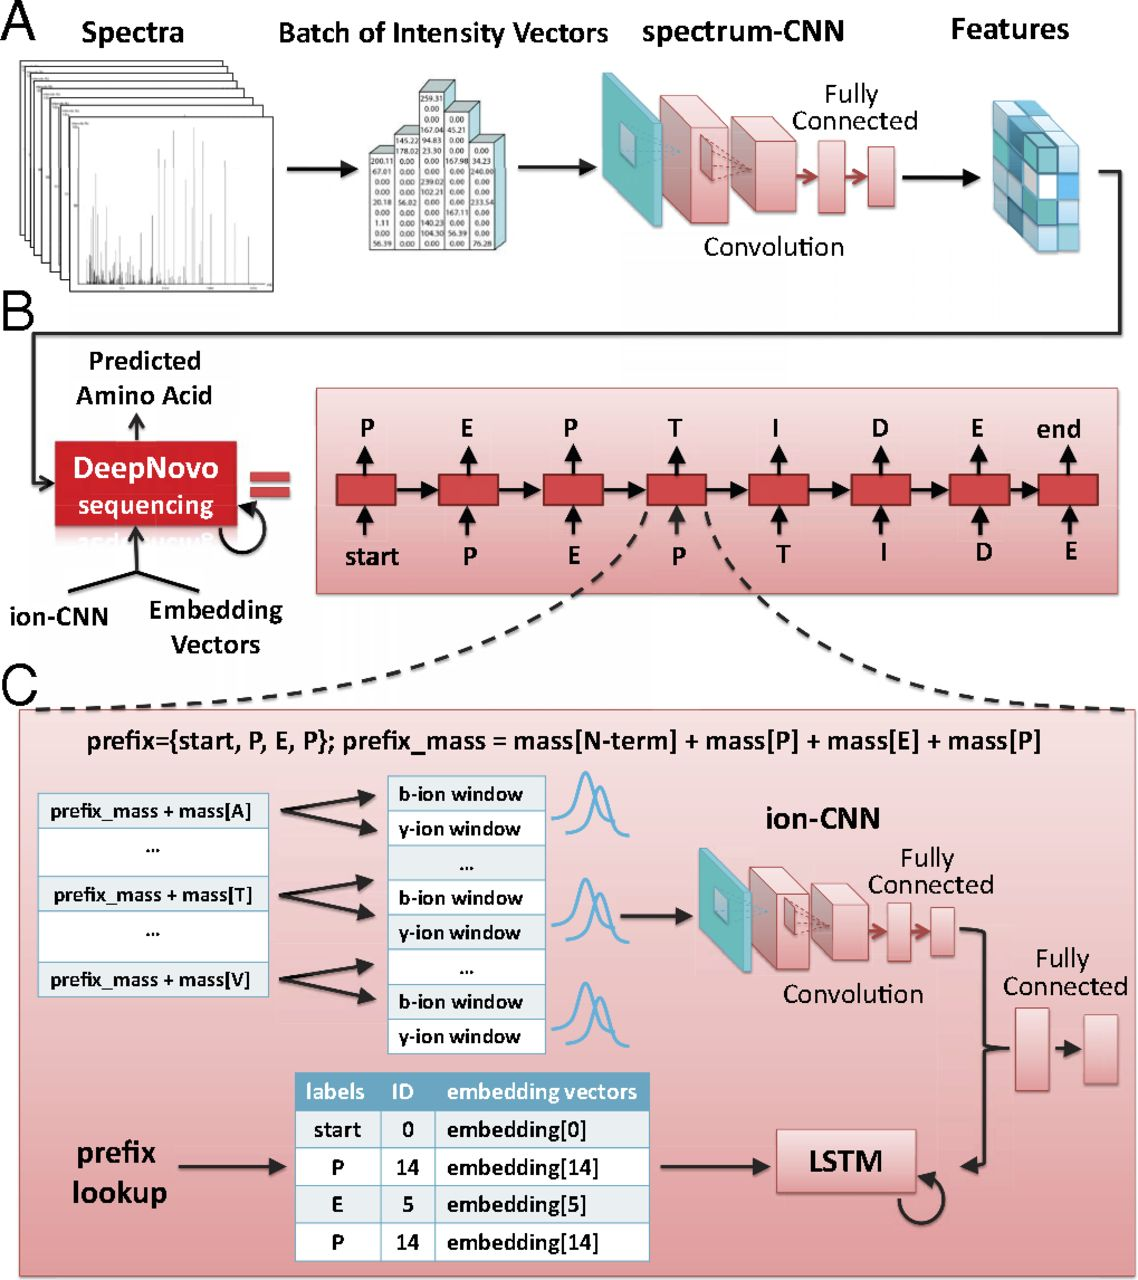
\includegraphics[width=0.8\textwidth]{images/deep_novo_architecture.jpeg}
\caption{Arhitektura DeepNovo pristupa, preuzeto sa \cite{deepnovo}}
\label{fig:arhitektura}
\end{figure}

\subsubsection{Konvolucione neuronske mreže (CNN)}
\textbf{CNN} se koristi za otkrivanje značajnih šablona u ulaznim podacima. Veoma je efikasna mreža i koristi tehniku \emph{sliding window} i procesuira male lokalne regione koristeći filtere. U slučaju \textbf{DeepNovo} tehnike, konvoluciona mreža se sastoji od 3 konvoluciona sloja i koristi \emph{ReLu} aktivacionu funkciju. Ova mreža je trenirana da prepozna lokalne šablone, različite tipove jona i da pretvori sirove podatke u reprezentaciju svojstava ulaznih podataka.

U ovom modelu su korišćene 2 \textbf{CNN} mreže:

\begin{itemize}
\item \textbf{Spektralna CNN}: Spektar dobijen masenom spektrometrijom konvertuje u vektor fiksne dužine (koji obično ima od 50 do 100 hiljada elemenata) i dobijeni vektor se prosleđuje ovoj mreži. Ovime se uče šabloni nad svim podacima spektrometrije i rezultat ove mreže se dalje koristni u rekurentnoj mreži. Ovo predstavlja značajan deo arhitekture jer može dosta da poboljša preciznost sekvenciranja i može da nauči šablone u spektru čak i ako su neki peak-ovi pomereni u spektru zbog šuma.
\item \textbf{Jonska CNN}: Ova mreža se koristi tokom odabira sledeće aminokiseline u peptidu i ona služi da za mali region spektralnih podataka izvuče najbitnije informacije. Gleda da li za predviđenu aminokiselinu postoje očekivani fragmenti jona. Prilikom svakog koraka predviđanja sledeće aminokiseline \textbf{DeepNovo} generiše teorijski spektar fragmenata uz pomoć prefiksnih masa. Za svaki jon izvlači se mali prozor iz spektra oko tog jona i na kraju se dobije više različitih ulaza u mrežu. Ovaj deo modela je bitan u slučaju da su podaci šumoviti ili da neki vrh spektra nedostaje.
\end{itemize}

\subsubsection{Rekurentne neuronske mreže (RNN)}
Ove mreže su dizajnirane za predviđanje sekvenci, gde izlaz zavisi ne samo od trenutne tačke podataka (podaci masenog spektra) već i od prethodnih tačaka podataka. U kontekstu sekvenciranja peptida, \textbf{RNN} može naučiti kako jedna aminokiselina utiče na sledeću u sekvenci, što je ključno za tačno predviđanje.

\emph{DeepNovo} koristi posebnu vrstu RNN-a koja se zove \emph{Long Short-Term Memory (LSTM)}. Ključna prednost \textbf{LSTM} mreža je ta što bolje prati duže zavisnosti, konkretno peptidi mogu da budu različitih dužina a ova mreža pamti i odnose koji su udaljeni, odnosno početak sekvence može da utiče na predviđanje neke kasnije aminokiseline.

Ova mreža se sastoji od 1 sloja \textbf{LTSM}-a i radi tako što dodaje jednu po jednu aminokiselinu sve dok ne stigne do kraja peptida. U svakom koraku \textbf{LTSM} mreža gleda:
\begin{itemize}
    \item Šta je mreža naučila do sada - trenutno stanje
    \item Sledeća aminokiselina koja je kandidat
    \item Svojstva spektra koja su dobijana od konvolucione mreže
\end{itemize}

Na osnovu ovoga, mreža određuje koja ja verovatnoća da je trenutna aminokiselina zapravo nalazi na datoj poziciji u peptidu.

Kao izlaz iz ove mreže koristi se \emph{softmax} projekcija i ona određuje za svaku aminokiselinu koja je verovatnoća da se ona nalazi na sledećoj poziciji u sekvenci. Dodatno, koristi se \emph{beam search}, odnosno ne bira se samo aminokiselina sa najvećom verovatnoćom nego se čuva više kandidata koji imaju veću verovatnoću. Ovim postupkom se povećava preciznost i gledaju se alternativna rešenja. Na kraju se sekvence rangiraju po rezultatu koliko se poklapaju sa traženim spektrom i koliko imaju grešaka i bira najbolja moguća.

\subsection{Rezultati i evaluacija}

\emph{DeepNovo} metoda nadmašuje tradicionalne metode, posebno u slučajevima kada su sekvence peptida nove i ne podudaraju se ni sa jednom poznatom proteinskom bazom podataka.

Eksperimenti su pokazali značajno poboljšanje u tačnosti identifikacije aminokiselina, posebno za složene peptide.

Za potrebe testiranja naučnici su koristili podatke različitih vrsta. Na slici \ref{fig:performanse} su prikazani rezultati poređenja više algoritama. Da bi se merila preciznost rešenja poređena je prava sekvenca aminokiselina sa onom koja je dobijena na osnovu spektra. 
Takođe, koristile su se različite metrike:
\begin{itemize}
    \item \textbf{Preciznost (eng. precision)} - koji predstavlja broj peptida koji je generisao algoritam koji su zapravo tačni
    \item \textbf{Odziv (eng. recall)} - koji broj stvarnih peptida je uspešno pronađen od strane modela
    \item \textbf{AUC-PR} - koliko dobro model balansira preciznost i odziv, što veća vrednost bolje će biti i preformanse
\end{itemize}

Može se primetiti da je \textbf{DeepNovo} model na svakom od datih skupa podataka imao bolje rezultate. \textbf{DeepNovo} je imao i veću preciznost u traženju peptida kao i veći odziv, samim tim i odnos \emph{AUC-PR} krive je bolji nego kod konkurenata.

\begin{figure}[h]
\centering
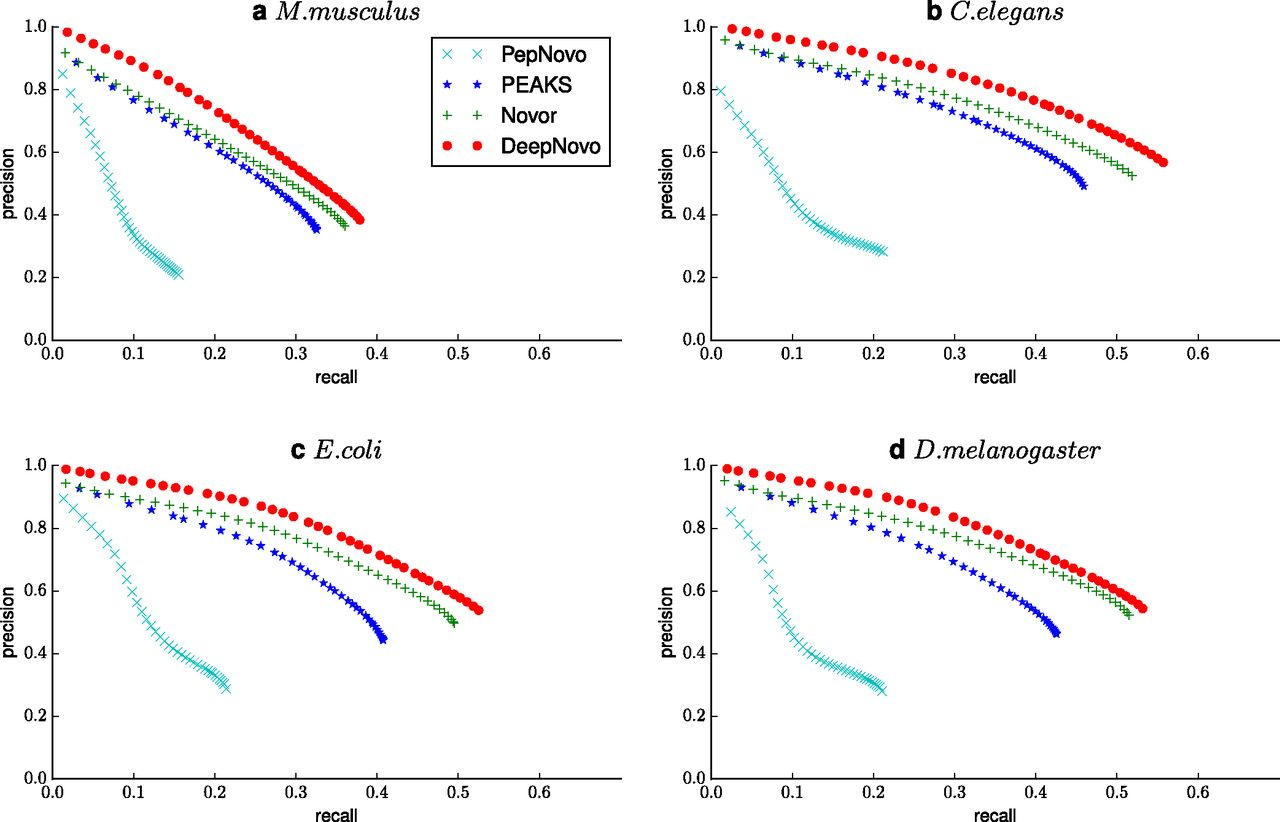
\includegraphics[width=0.8\textwidth]{images/deep_novo_comparison.jpeg}
\caption{Poređenje performansi DeepNovo sa drugim algoritmima, preuzeto sa \cite{deepnovo}}
\label{fig:performanse}
\end{figure}

\textbf{DeepNovo} je uspešno primenjen u nekoliko realnih scenarija:

\begin{itemize}
\item \textbf{Identifikacija novih antimikrobnih peptida}: Otkrivanje potencijalnih kandidata za nove antibiotike
\item \textbf{Analiza post-translacionih modifikacija}: Detekcija peptida sa složenim modifikacijama koje su se desile nakon njegovog kreiranja
\item \textbf{Univerzalna primena}: Uspešna implementacija na različitim vrstama i organizmima
\end{itemize}


% ------------------------------------------------------------------------------
\chapter{Elektronska platforma}
% ------------------------------------------------------------------------------

U ovom poglavlju će biti opisana elektronska platforma koja je napravljena kao deo ovog rada. Objasniće se njeno pokretanje i korišćenje kao i tehnologije koje su korišćene prilikom pravljenja platforme.

\emph{Frontend} aplikacije je pisan u programskom jeziku \textbf{TypeScript} \cite{typescript} uz korišćenje \textbf{Node 18} \cite{node} i \textbf{Next.js} \emph{framework}-a \cite{next}.
\emph{Backend} aplikacije je implementiran u programskom jeziku \textbf{Python 3.12} \cite{python} uz korišćenje \textbf{Django} \emph{framework}-a \cite{django}. Izvorni kod aplikacije se nalazi na \emph{GitHub}-u, u javnom repozitorijumu \cite{github}.

\section{Pokretanje aplikacije}

Pokretanje aplikacije može da se odradi na nekoliko načina:
\begin{itemize}
    \item \textbf{Docker Compose} \cite{docker_compose} - najjednostavniji način pokretanja aplikacije uz korišćenje \emph{Docker} alata \cite{docker}
    \item \textbf{Direktno pokretanje komponenti} - pokretanje posebno \emph{Frontend} i posebno \emph{Backend} komponenti
    \item \textbf{Google Cloud Run (GCR)} \cite{gcr} - ova aplikacija je dostupna za korišćenje preko \emph{Google Cloud Run} platforme, pa će se samim tim objasniti i kako odraditi \emph{deploy} aplikacije na \textbf{GCR}
\end{itemize}

\subsection{\emph{Docker Compose} konfiguracija}
Za potrebe što lakšeg pokretanja aplikacije korišćen je \emph{open source} alat \emph{Docker} i \emph{Docker Compose}. \emph{Docker Compose} nam pruža jednostavan način da aplikaciju pokrenemo sa svim definisanim bibliotekama, promenljivama okruženja bez potrebe da se bilo šta dodatno namesti. Ovo je posebno bitno u slučaju kada se aplikacija sastoji iz više komponenti pa je potrebno da se pokrene više kontejnera kao što je ovde slučaj.
Unutar \textbf{docker} foldera nalaze \emph{docker} i \emph{docker-compose fajlovi}.

Što se tiče klijentskog dela aplikacije njegovo pokretanje je definisano u \emph{Dockerfile.frontend} datoteci i njegov sadržaj može da se vidi na slici \ref{fig:docker_frontend}.

\begin{figure}[h]
\centering
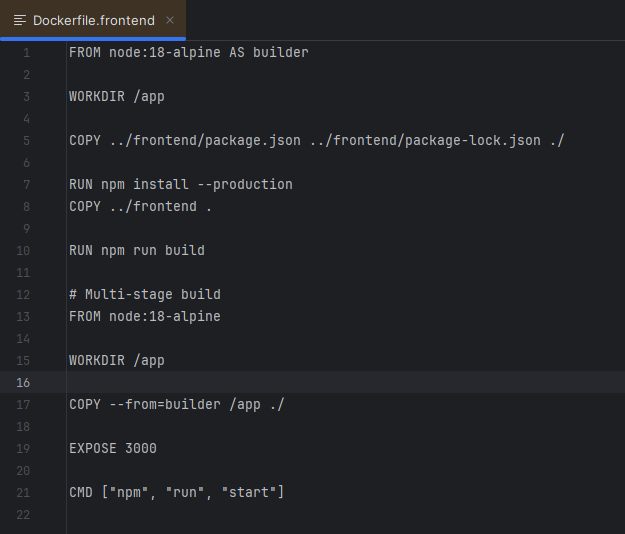
\includegraphics[width=0.9\textwidth]{images/docker_frontend.png}
\caption{\emph{Dockerfile} za klijentski deo aplikacije}
\label{fig:docker_frontend}
\end{figure}

Može da se primeti da se koristi \emph{multi-stage build} koji služi da odvoji deo za instaliranje i kompilaciju fajlove od dela koji će pokrenuti aplikaciju. Ovo doprinosi tome da završa slika bude što manja.

Pokretanje serverskog dela aplikacije definisano je u \emph{Dockerfile.backend} datoteci i njegov sadržaj može da se vidi na slici \ref{fig:docker_backend}.

\begin{figure}[h]
\centering
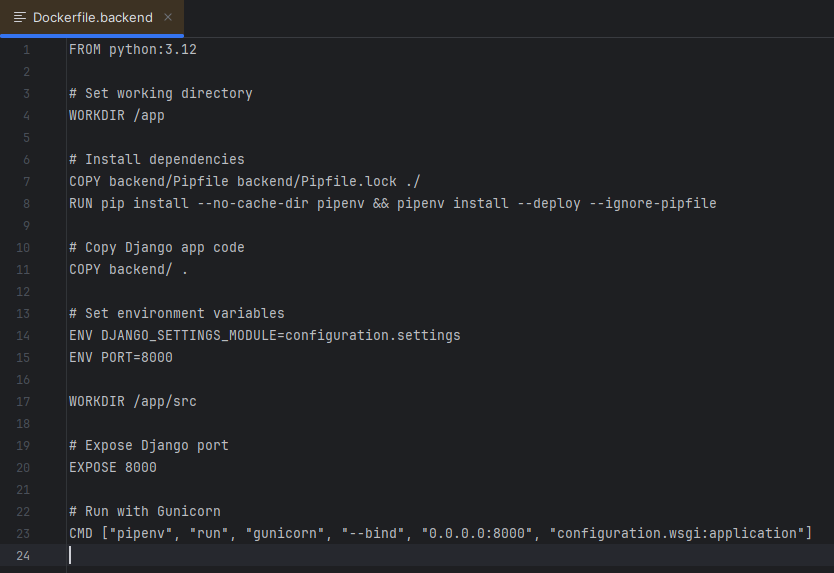
\includegraphics[width=0.9\textwidth]{images/docker_backend.png}
\caption{\emph{Dockerfile} za serverski deo aplikacije}
\label{fig:docker_backend}
\end{figure}

Može da se primeti da se koristi \emph{Gunicorn} koji predstavlja \emph{WSGI HTTP} server za produkciona okruženja.

Sadržaj glavne \texttt{docker-compose.yml} datoteke može da se vidi na slici \ref{fig:docker_compose}.

\begin{figure}[h]
\centering
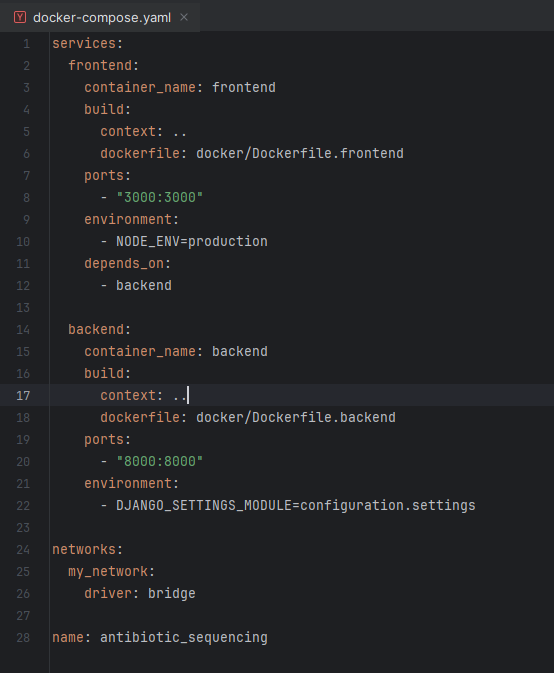
\includegraphics[width=0.9\textwidth]{images/docker_compose.png}
\caption{\emph{Docker Compose} fajl koji pokreće definisane \emph{Docker} fajlove}
\label{fig:docker_compose}
\end{figure}

Da bi se projekat pokrenuo potrebno je pozicionirati se u \textbf{/docker} direktorijum i pokrenuti sledeću komandu:
\begin{verbatim}
    docker-compose up -d --build
\end{verbatim}

Ova komanda pokreće dva kontejnera. \emph{Frontend} delu aplikacije može da se pristupi tako što se u veb pregladaču otvori \emph{http://localhost:3000}, dok se \emph{backend} deo aplikacije nalazi na \emph{http://localhost:8000}.

\subsection{Direktno pokretanje komponenti}

Da bi se direktno pokrenuo \emph{Frontend} aplikacije potrebno je imati instaliran \textbf{Node 18} kao i \textbf{npm 10} paket menadžer. Potrebno je pozicionirati se u \textbf{/frontend} direktorijum i pokrenuti naredne komande:
\begin{verbatim}
    npm install
    npm run build
    npm run start
\end{verbatim}

Nakon pokretanja ovih komandi klijentskom delu aplikacije može da se pristupi iz veb pregledača na adresi \emph{http://localhost:3000}.

Da bi se direktno pokrenuo \emph{Backend} aplikacije potrebno je imati instaliran \textbf{Python 3.12} kao i \textbf{pip} paket menadžer. Potrebno je pozicionirati se u \textbf{/backend} direktorijum i izvršiti naredne komande:  
\begin{verbatim}
    python -m venv venv
    venv\Scripts\activate
    pip install pipenv
    pipenv install -d
    cd src
    python manage.py runserver
\end{verbatim}

Pokretanjem ovih komandi kreiraćemo virtuelno okruženje u kom će se instalirati sve zavisnosti ove aplikacije. Za praćenje verzije korišćenih biblioteka korišćen je \emph{Pipfile} i zato mora da se instalira i \emph{pipenv}.
Nakon pokretanja serverskom delu aplikacije mogu se slati zahtevi na adresu \emph{http://localhost:8000}.

\subsection{\emph{Google Cloud Run} implementacija}
Aplikacija je trenutno \emph{deploy}-ovana na Google Cloud Run i može joj se pristupiti preko \emph{https://antibiotic-sequencing-304513663933.us-central1.run.app/}.
Koristi se besplatna verzija koja se ne naplaćuje a pored toga \emph{Google Cloud Run} pruža sledeće pogodnosti:

\begin{itemize}
\item \textbf{Skalabilnost}: Automatsko skaliranje u zavisnosti od opterećenja
\item \textbf{Integracija}: Potpuna podrška za \emph{Docker} kontejnere
\item \textbf{Bezbednost}: Ugrađena zaštita \emph{DDoS} napada
\item \textbf{Monitoring}: Integrisani \emph{Cloud Monitoring} alati
\end{itemize}

Postoji \emph{Google Cloud CLI} alat koji može da se instalira i da se iz terminala pokreću odgovarajuće komande. Proces se sastoji iz sledećih koraka i potrebno je da se ovi koraci odrade i za klijentsku i za serversku komponentu:

\begin{enumerate}
\item Pravljenje projekta na \emph{Google Cloud} platformi čiji će se \emph{PROJECT\_ID} dalje koristiti
\item Povezivanje \emph{Google Cloud CLI} alata sa \emph{Google} nalogom:
\begin{verbatim}
    gcloud auth login
\end{verbatim}
\item Definisanje sa kojim projektom želimo da radimo:
\begin{verbatim}
    gcloud config set project <PROJECT_ID>
\end{verbatim}
\item Pravljenje \emph{Docker} image-a:
\begin{verbatim}
    docker build -t gcr.io/<PROJECT_ID>/fe:v1.0 
    -f docker/Dockerfile.frontend .
\end{verbatim}
\item Kačenje slike na njihov repozitorijum:
\begin{verbatim}
    docker push-t gcr.io/<PROJECT_ID>/fe:v1.0
\end{verbatim}
\item Deploy servisa: 
\begin{verbatim}
    gcloud run deploy antibiotic-sequencing 
    --image gcr.io/<PROJECT_ID>/fe:v1.0 
    --platform managed 
    --region us-central1
    --allow-unauthenticated 
    --port 3000
\end{verbatim}
\end{enumerate}

Nakon toga u terminalu se dobija \emph{URL} na kom može da se pristupi podignutom servisu što se može videti na slici \ref{fig:gcr_deploy}. Takođe u toj situaciji frontend komponenti mora u \textbf{/.env} fajlu da se promeni \emph{URL} koji vodi do bekend komponente.

\begin{figure}[h]
\centering
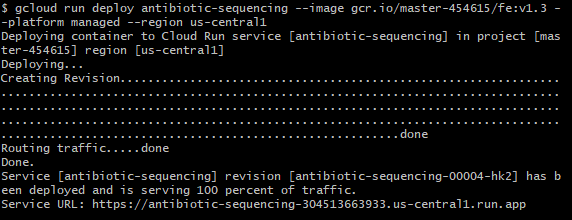
\includegraphics[width=0.9\textwidth]{images/gcr_deploy.png}
\caption{Dobijeni \emph{URL} nakon što se aplikacija podigne na \emph{Google Cloud Run} servisu}
\label{fig:gcr_deploy}
\end{figure}

U slučaju da je potrebno okačiti novu verziju aplikacije, prate se isti koraci za pravljenje i kačenje slike dok se komanda za \emph{deploy} razlikuje jer se navodi kako se zove komponenta koja se ažurira:
\begin{verbatim}
    gcloud run deploy antibiotic-sequencing 
    --image gcr.io/<PROJECT_ID>/fe:v1.1 
    --platform managed 
    --region us-central1
\end{verbatim}

Ako želimo da pristupimo \emph{Docker} slikama koje smo okačili potrebno je otvoriti \emph{https://console.cloud.google.com/artifacts}, slika \ref{fig:gcr_images}.
\begin{figure}[h]
\centering
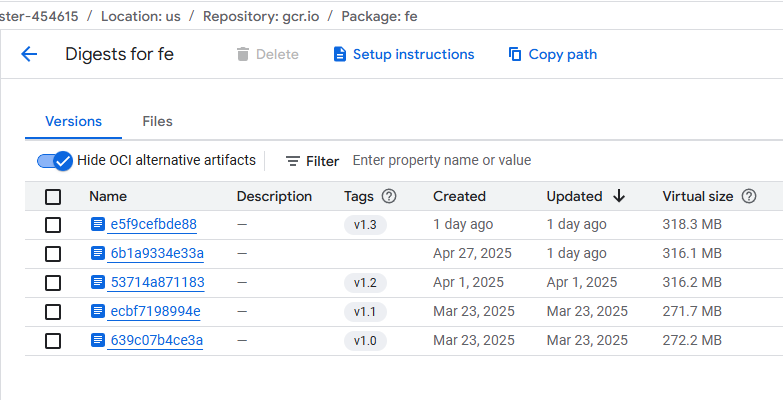
\includegraphics[width=0.9\textwidth]{images/gcr_images.png}
\caption{\emph{Docker} slike koje su okačene na \emph{Google Container Registry}}
\label{fig:gcr_images}
\end{figure}

Podignutim servisima može se pristupiti preko \emph{https://console.cloud.google.com/run}, slika \ref{fig:gcr_services}.

\begin{figure}[h]
\centering
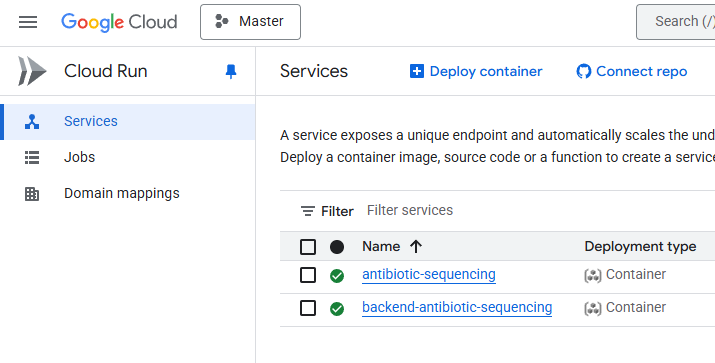
\includegraphics[width=0.9\textwidth]{images/gcr_services.png}
\caption{Pristupi servisima koji su podignuti na \emph{Google Cloud Run} platformi}
\label{fig:gcr_services}
\end{figure}

Ako se klikne na neki od servisa pristupiće se brojnim metrikama koje su nam dostupne, \ref{fig:gcr_services_details}. Takođe, tu možemo da vidimo i koji je \emph{URL} našeg servisa kao i da vidimo koji je status i da li su se desile neke greške.

\begin{figure}[h]
\centering
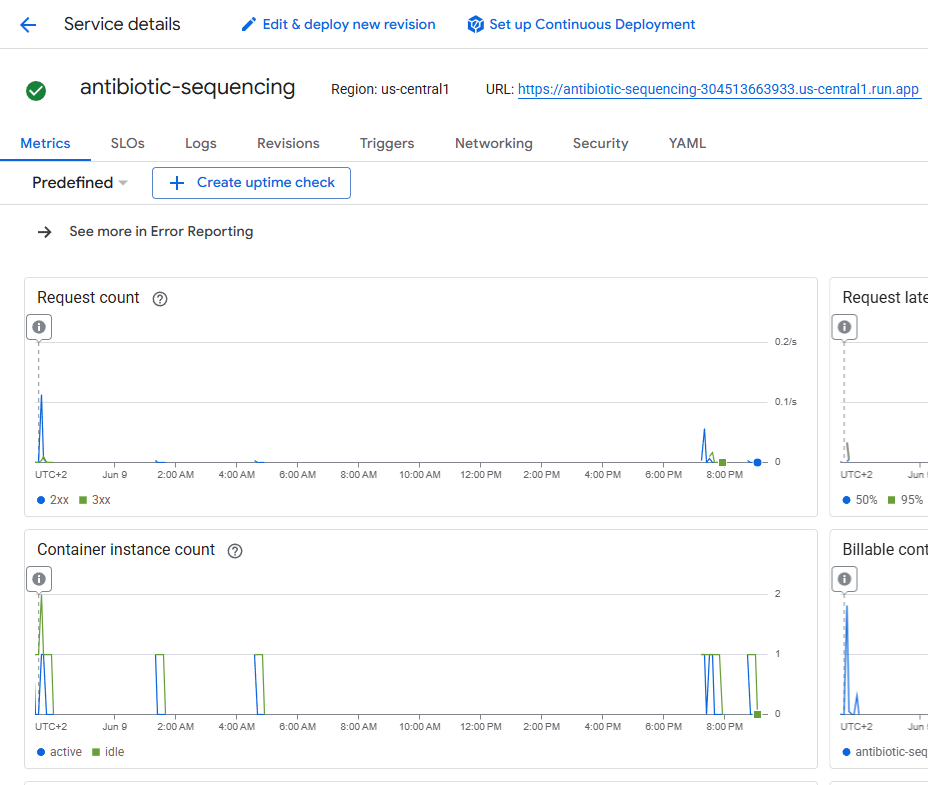
\includegraphics[width=0.9\textwidth]{images/gcr_services_details.png}
\caption{Detalji i metrike koje su nam dostupne kada pristupimo nekom servisu}
\label{fig:gcr_services_details}
\end{figure}


\section{Funkcionalnosti platforme}

\subsection{Početna stranica}

Prilikom otvaranja aplikacije otvoriće se početna stranica koja može da se vidi na slici \ref{fig:landing_page}. Na vrhu stranice nalazi se navigacioni meni kojim može da se prelazi sa stranice na stranicu. Takođe, u gornjem desnom uglu nalazi se ikonica koja vodi ka \emph{Github} repozitorijumu gde može da se nađe izvorni kod ove aplikacije.
Klikom na dugme \emph{Istraži algoritme} odlazi se na stranicu \emph{Uvod}, gde mogu da se nađu teorijska objašnjenja pojma koja su potrebna za razumevanje algoritama.

\subsection{Uvodna stranica}

Ova stranica služi da predstavi teorijske osnove i pojmove koji su potrebni za dalje razumevanje algoritama. Na slici \ref{fig:intro_1} može da se vidi deo ove stranice. Klikom na bilo koju sliku sa ove stranice ona će se otvoriti i omogućiti jasniji prikaz iste.

Na dnu stranice stranice, koja je prikazana na slici \ref{fig:intro_2}, takođe postoji meni koji vodi ka algoritmima koji su odrađeni u sklopu ovde aplikacije.

\begin{figure}[H]
\centering

\includegraphics[width=1\textwidth]{images/landing_page.png}
\caption{Početna stranica kada se otvori aplikacija}
\label{fig:landing_page}
\end{figure}

\begin{figure}[H]
\centering
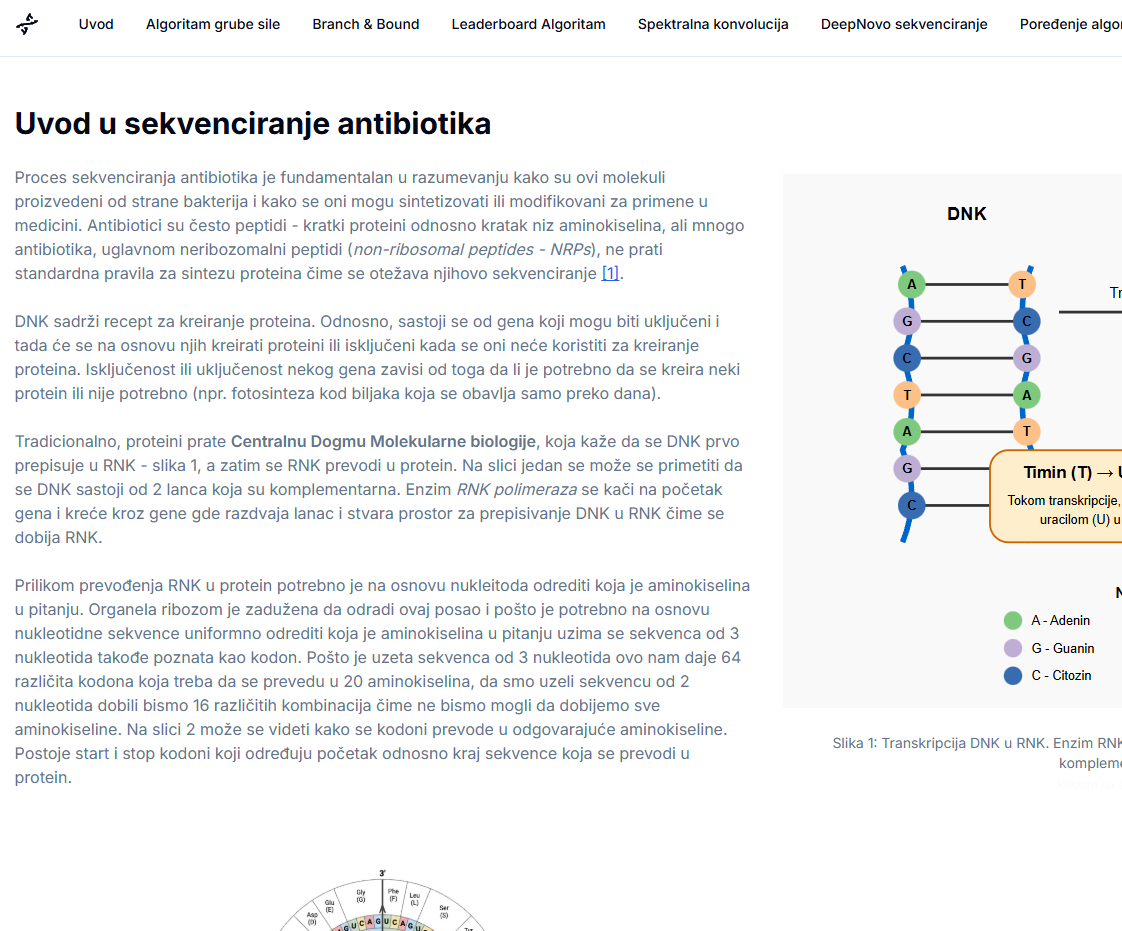
\includegraphics[width=1\textwidth]{images/intro_1.png}
\caption{Uvodna stranica sa teorijskim pojmovima}
\label{fig:intro_1}
\end{figure}

\begin{figure}[H]
\centering
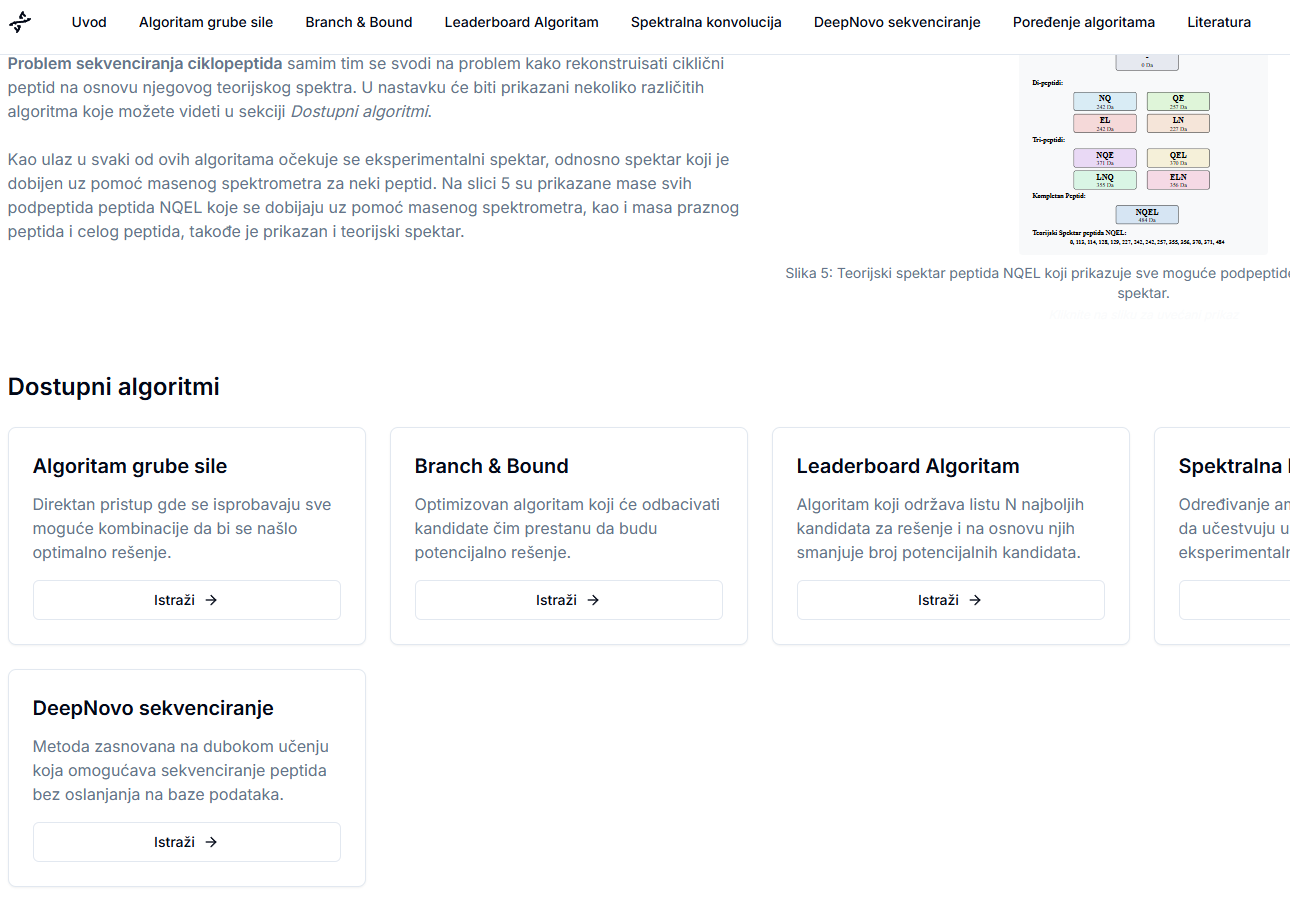
\includegraphics[width=1\textwidth]{images/intro_2.png}
\caption{Navigacioni meni na dnu Uvodne stranice koji vodi ka algoritmima}
\label{fig:intro_2}
\end{figure}

\subsection{Algoritam grube sile}

Stranica za algoritam grube sile, na slici \ref{fig:brute_force_1}, sadrži objašnjenje ovog algoritma kao i kod u programskom jeziku \emph{Python} za implementaciju algoritma.
\begin{figure}[h]
\centering
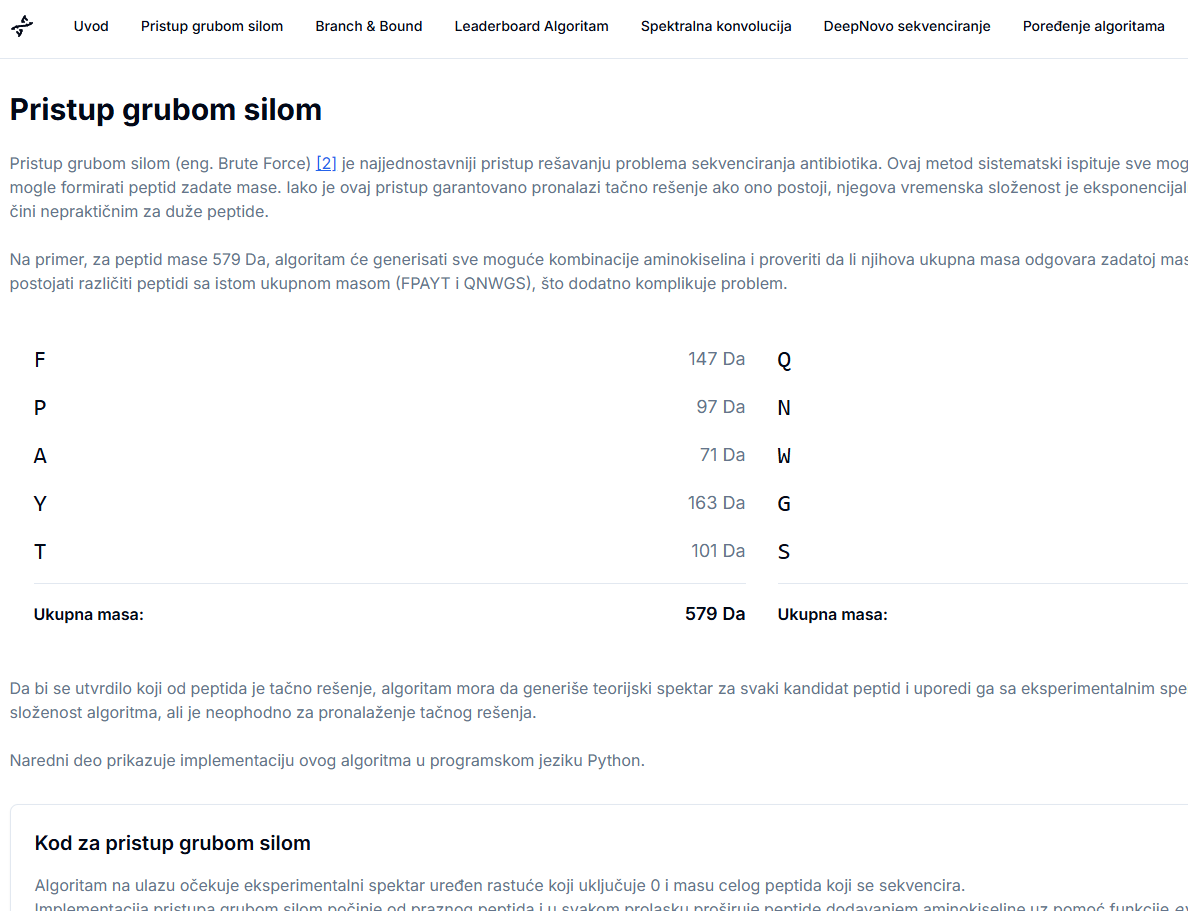
\includegraphics[width=1\textwidth]{images/brute_force_1.png}
\caption{Stranica za algoritam grube sile sa objašnjem istog}
\label{fig:brute_force_1}
\end{figure}

Nakon objašnjenja i koda za algoritam može da se unese eksperimentalni spektar i postoji mogućnost da se odabere da li korisnik želi da vidi vizuelizaciju ovog algoritma ili želi da vidi samo rešenja \ref{fig:brute_force_2}. Na slici \ref{fig:brute_force_4} može da se vidi drvo koje se izgradilo da bi se došlo do rešenja. Postoje i elementi za kontrolisanje izvršavanja animacije kao što su \emph{Play/Pause/Reset} a pored toga postoji i \emph{slider} kojim može da se premota animacija do određenog dela izvršavanja. Pošto drvo izvršavanja može da bude veoma veliko dodata je i opcija uveličavanja tako da određeni deo drveta može da se uveliča a onda ostatak drveta može da se vidi povlačenjem miša. Čvorovi koji su obeleženi zelenom bojom predstavljaju rešenje a crveni čvorovi su odbačeni i ne predstavljaju rešenje. Kada se miš postavi iznad nekog crvenog čvora prikazaće se i objašnjenje zašto on nije rešenje.
Kada se animacija završi moguće je kliknuti i na dugme \emph{Download} čime će se izgrađeno drvo skinuti na Vaš računar u \emph{SVG} formatu.
\clearpage
\begin{figure}[H]
\centering
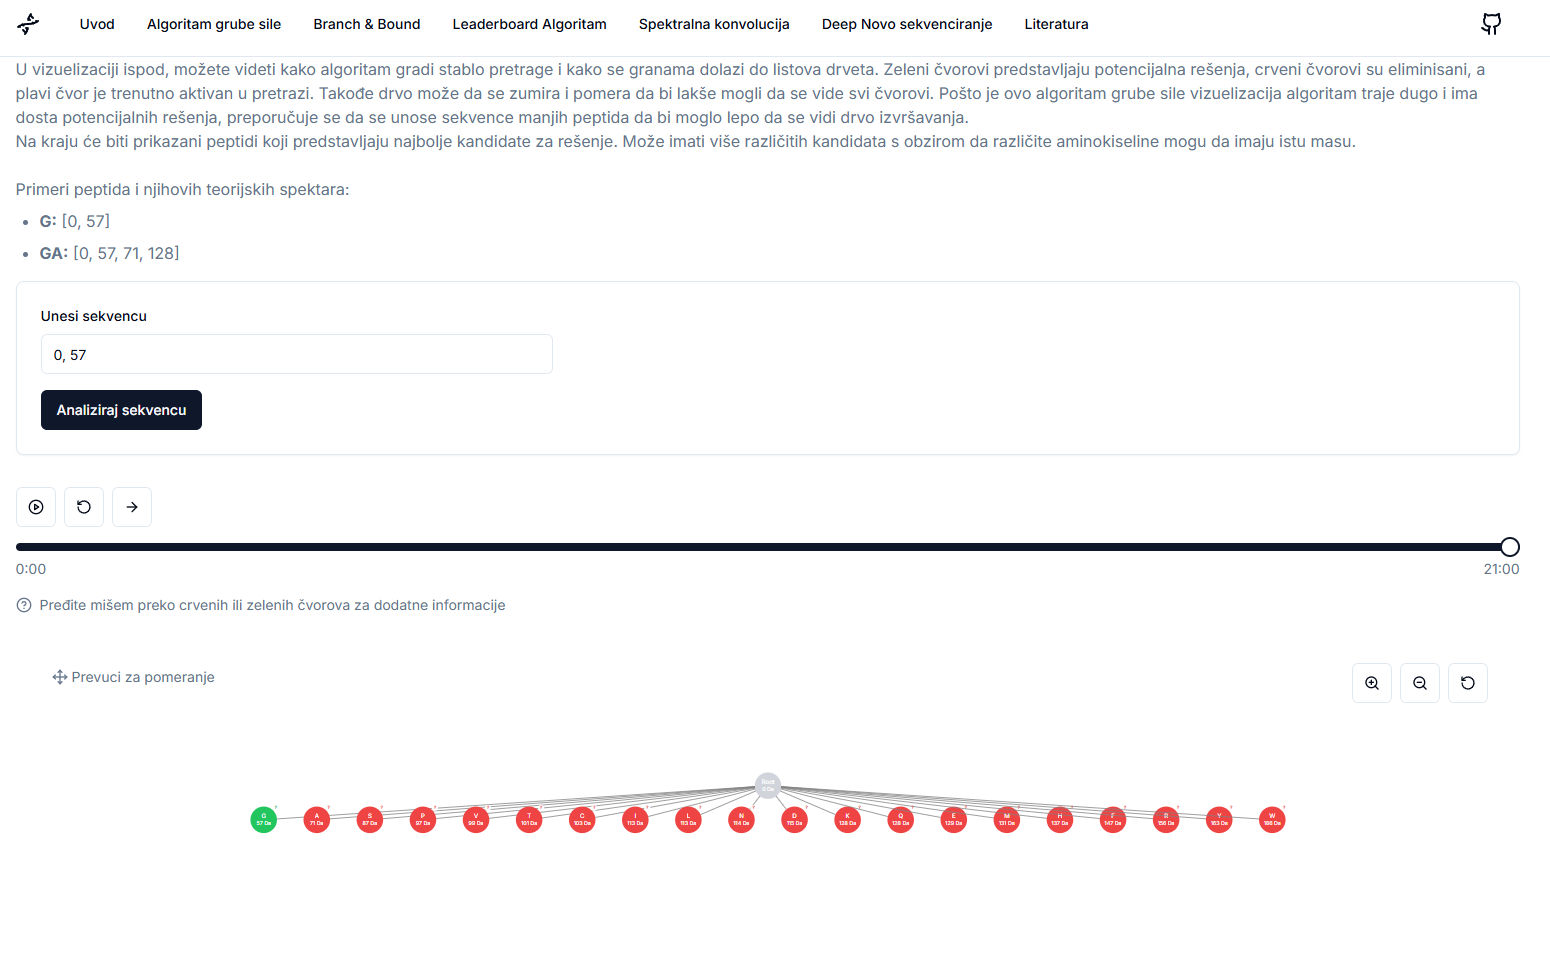
\includegraphics[width=0.5\textwidth]{images/brute_force_2.png}
\caption{Ulazna forma za eksperimentalni spektar sa opcijom da se označi da li se želi vizuelizacija ili ne}
\label{fig:brute_force_2}
\end{figure}

\begin{figure}[H]
\centering
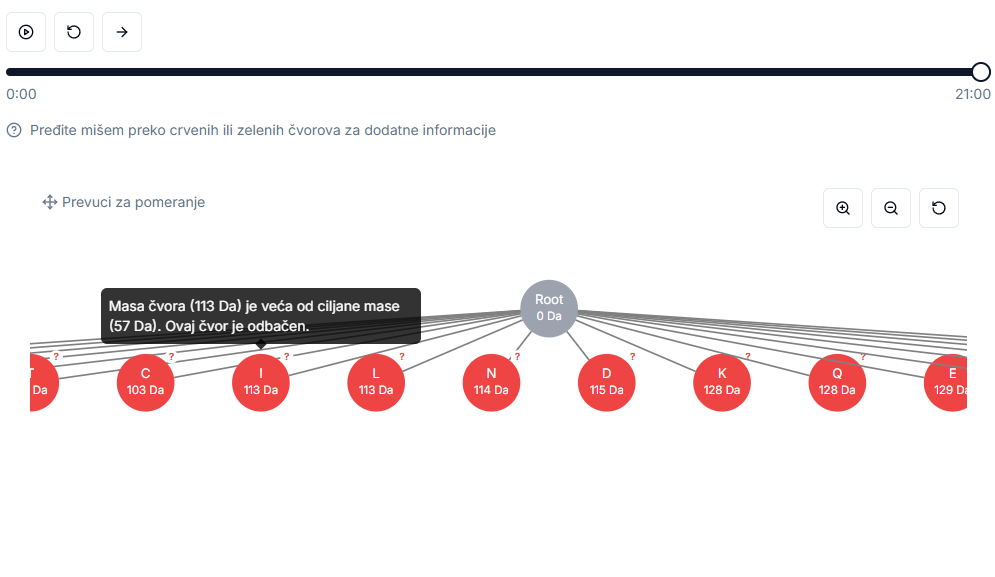
\includegraphics[width=1\textwidth]{images/brute_force_4.png}
\caption{Deo izgrađenog stabla u algoritmu grube sile}
\label{fig:brute_force_4}
\end{figure}

Na kraju će se za svaki peptid koji je kandidat da bude rešenje prikazati i njegov teorijski spektar a u slučaju da se taj teorijski spektar poklapa sa unetim eksperimentalni spektar prikazaće se poruka da je pronađeno rešenje, što se može videti i na slici \ref{fig:brute_force_3}. U slučaju da za zadati eksperimentalni spektar nema rešenja ispisaće se poruka koja to i govori.

\begin{figure}[H]
\centering
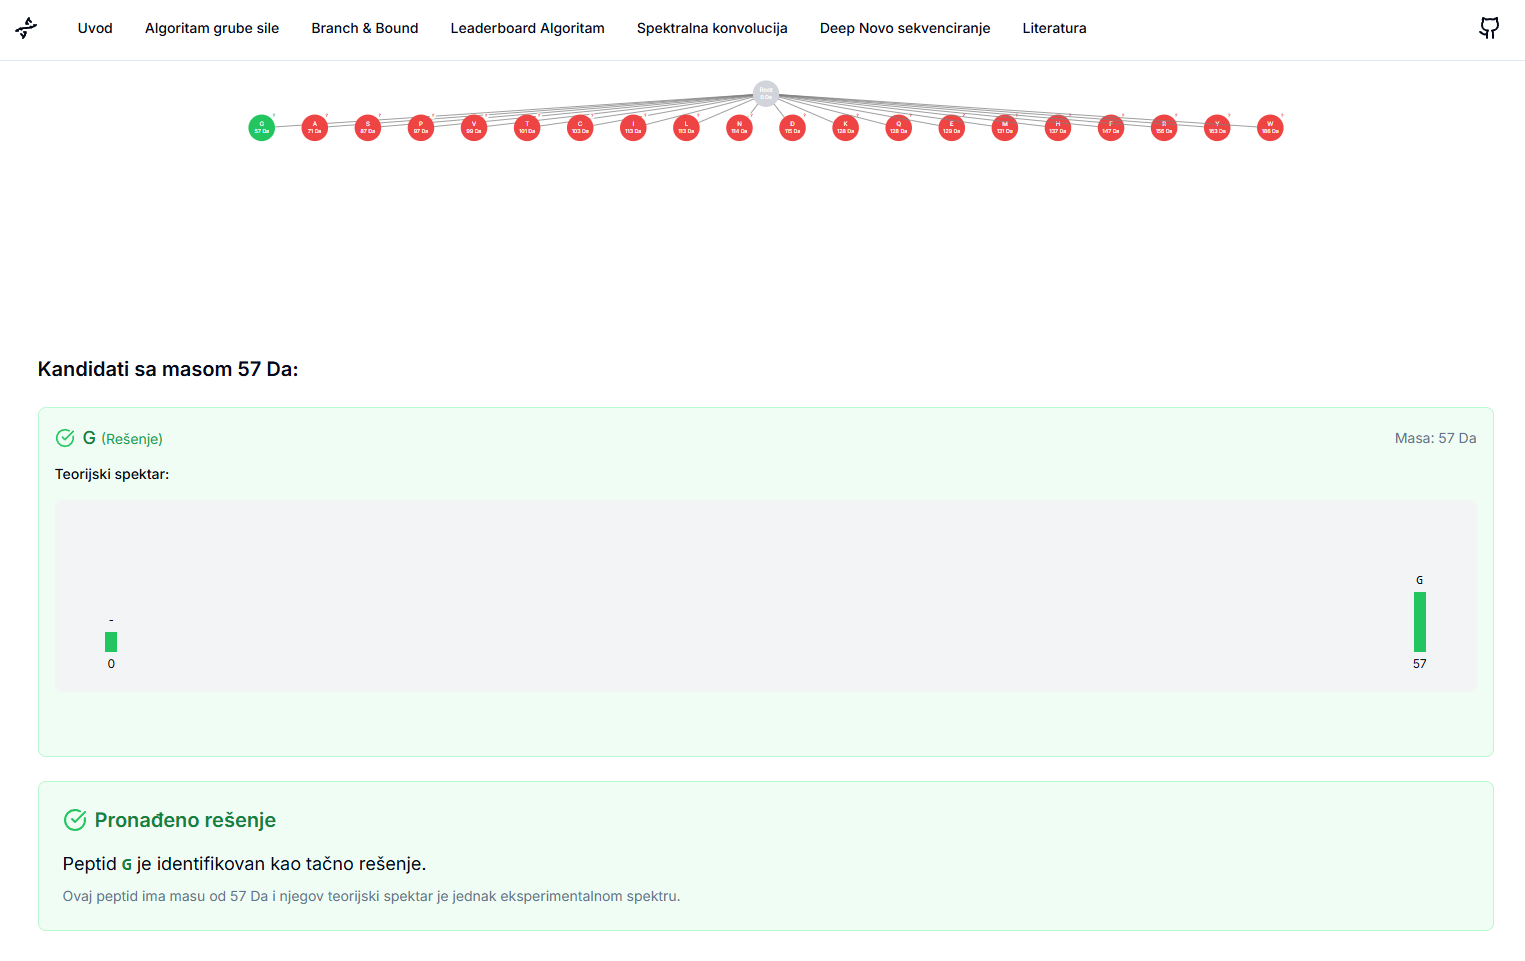
\includegraphics[width=1\textwidth]{images/brute_force_3.png}
\caption{Pronađena rešenja u algoritmu grube sile}
\label{fig:brute_force_3}
\end{figure}

\subsection{\emph{Branch and Bound}}
Stranica za algoritam \emph{Branch and Bound}, na slici \ref{fig:branch_and_bound}, sadrži objašnjenje ovog algoritma kao i kod u programskom jeziku \emph{Python} za implementaciju algoritma.
\begin{figure}[h]
\centering
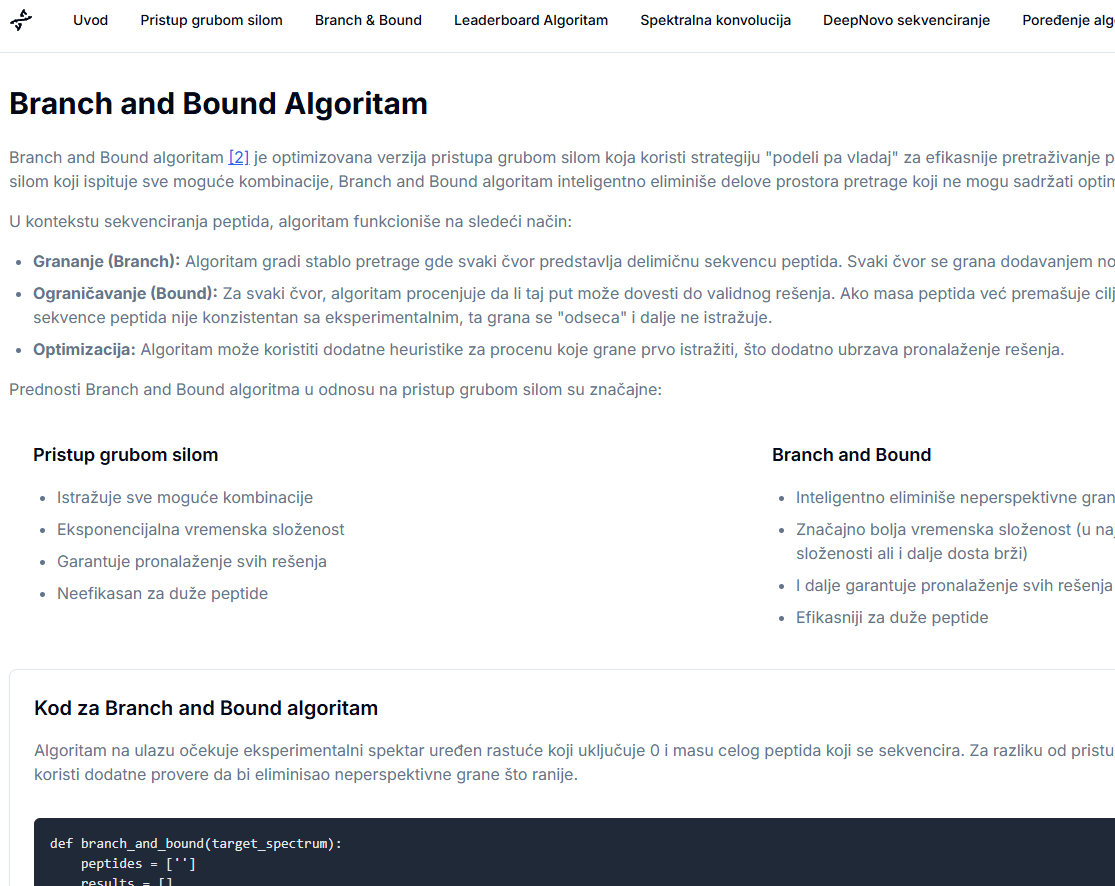
\includegraphics[width=1\textwidth]{images/branch_and_bound.png}
\caption{Stranica za algoritam Branch and Bound sa objašnjem istog}
\label{fig:branch_and_bound}
\end{figure}

Nakon objašnjenja i koda za algoritam može da se unese eksperimentalni spektar i može da se odabere da se vidi vizuelizacija ovog algoritma ili samo rešenje. Ovaj algoritam je veoma sličan algoritmu grube sile, tako da je i vizuelizacija i elementi koji čine tu vizuelizaciju potpuno ista. Jedina razlika je što je ovaj algoritam dosta brži i može da ranije odseče kandidate koji nisu rešenje tako da eksperimentalni spektar koji može da se unese je duži. Dodatno, pošto u ovom algoritmu postoji više razloga zašto je neki čvor odsečen tako će i poruke koje se prikazuju kada se mišem prevuče preko nekog čvora biti drugačije. Ovde je takođe po okončanju animacije moguće skinuti igrađeno drvo u \emph{SVG} formatu.

\subsection{\emph{Leaderboard}}
Stranica za algoritam \emph{Leaderboard}, na slici \ref{fig:leaderboard_1}, sadrži objašnjenje ovog algoritma kao i kod u programskom jeziku \emph{Python} za implementaciju algoritma.
\begin{figure}[H]
\centering
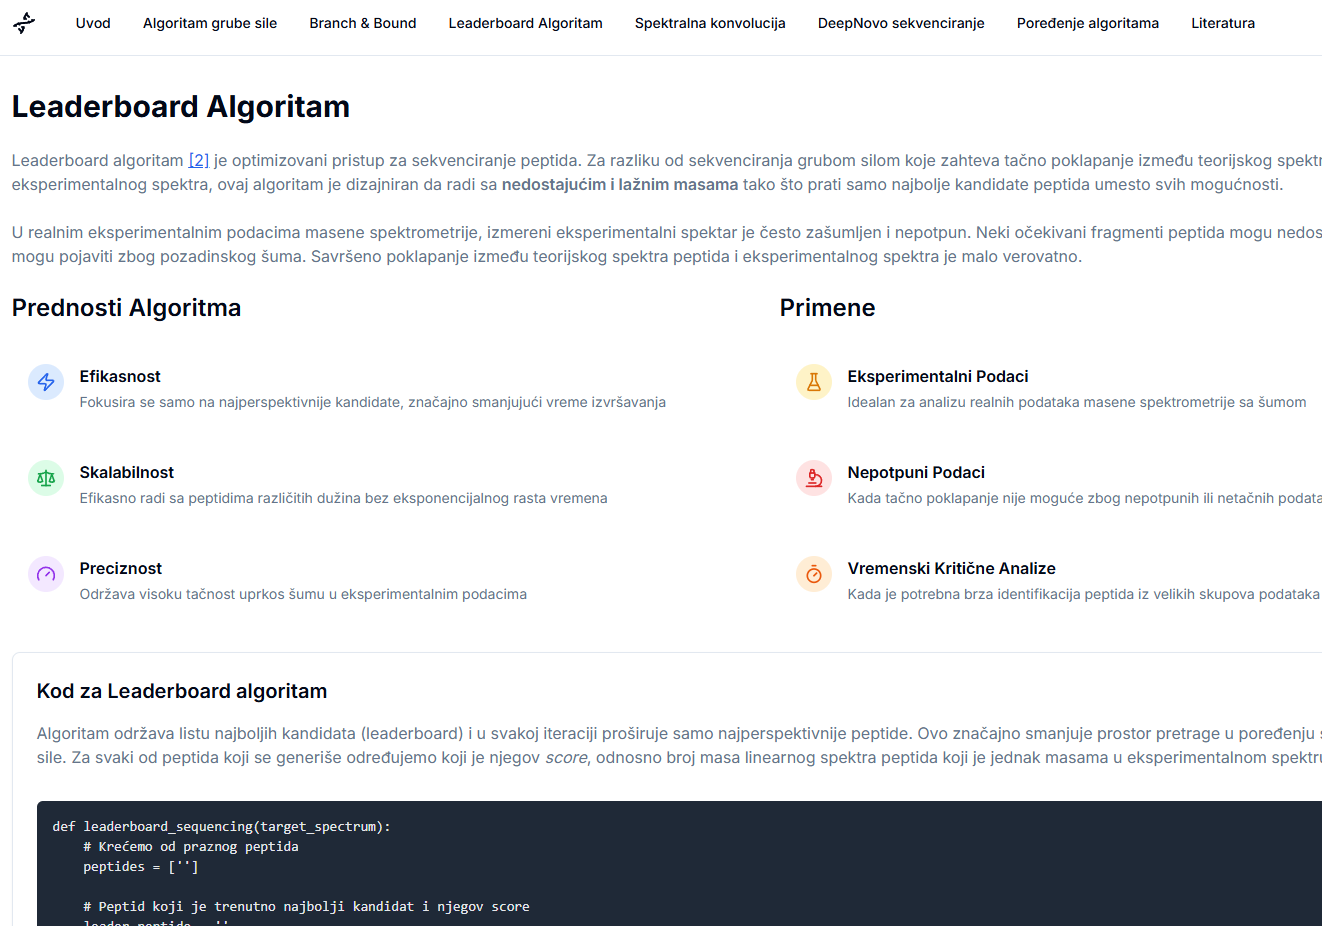
\includegraphics[width=1\textwidth]{images/leaderboard_1.png}
\caption{Stranica za algoritam Leaderboard sa objašnjem istog}
\label{fig:leaderboard_1}
\end{figure}

\begin{figure}[h]
\centering
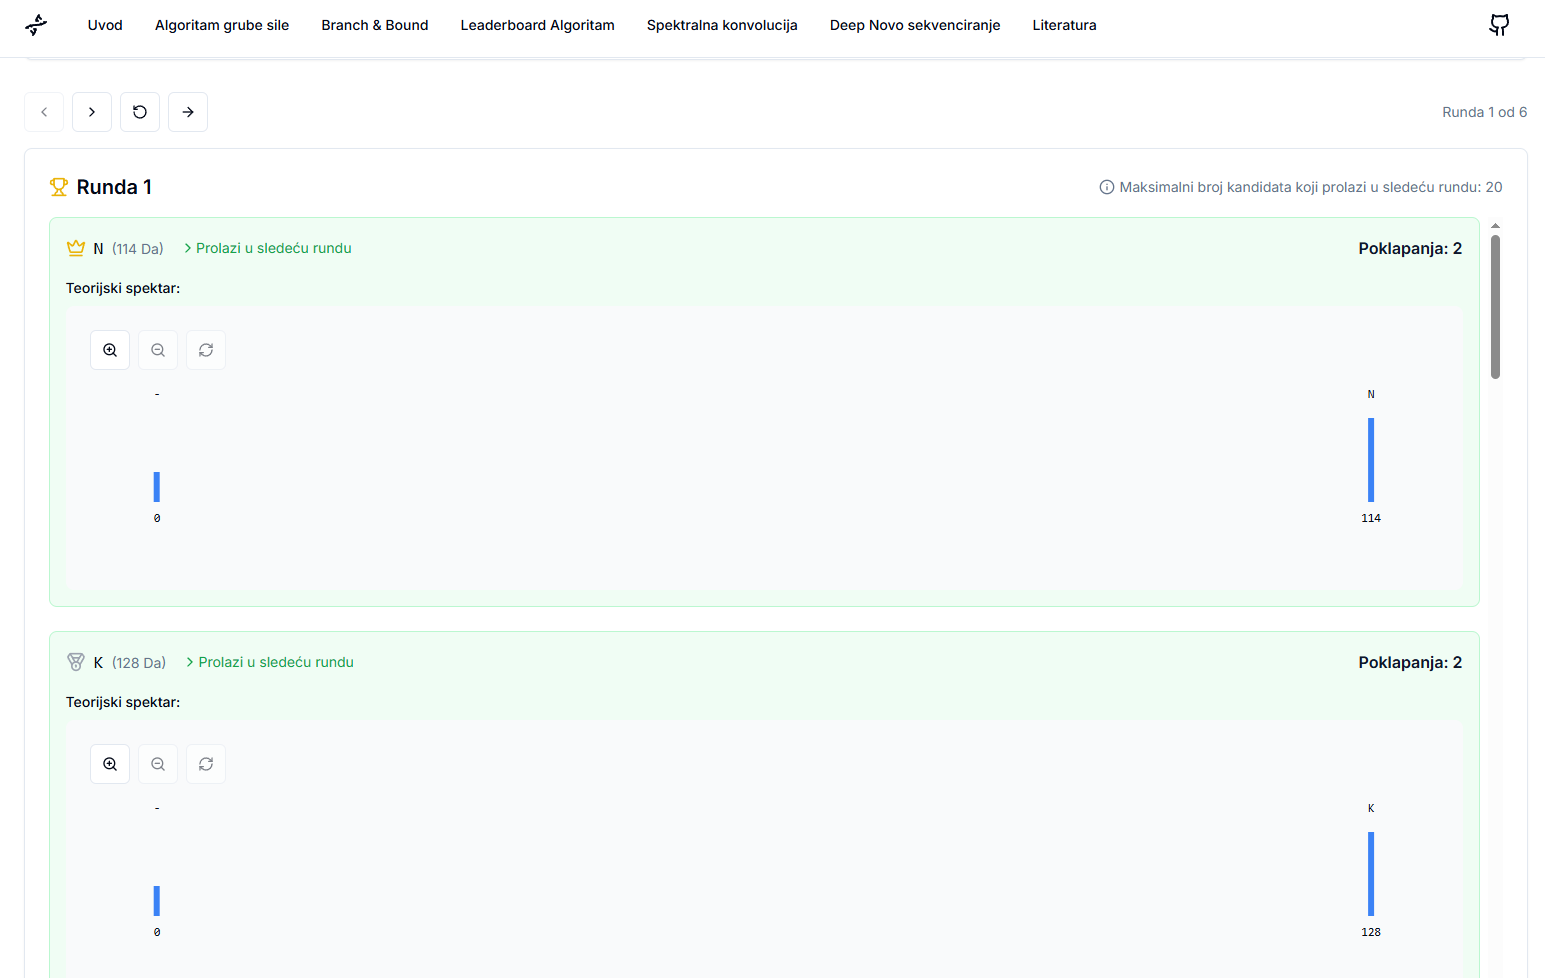
\includegraphics[width=1\textwidth,height=0.4\textheight]{images/leaderboard_2.png}
\caption{Prikaz rundi za Leaderboard algoritam}
\label{fig:leaderboard_2}
\end{figure}

Nakon objašnjenja i koda za algoritam može da se unese eksperimentalni spektar i može da se odabere da se vidi vizuelizacija ovog algoritma ili da se prikažu samo rešenja. Pošto ovaj algoritam funkcioniše po principu prolaska u sledeće runde vizuelizacija za ovaj algoritam je tako i odrađena što se može videti na slici \ref{fig:leaderboard_2}. Za kontrolu animacije postoje strelice za prebacivanje iz runde u rundu, strelica da nas prebaci skroz u poslednju rundu da bismo videli koje je rešenje kao i dugme za resetovanje odnosno prebacivanje na prvu rundu. Uz svaki peptid piše njegova masa, prikazuje se njegov teorijski spektar kao i broj poklapanja teorijskog spektra sa zadatim eksperimentalnim spektrom. Svaki peptid koji prolazi u sledeću rundu je označen zelenom bojom uz tekst da je prošao dalje.
Teorijski spektar svakog od peptida može da se uveliča po potrebi i da se koristi \emph{drag and drop} mehanizam da se vidi neki određeni deo spektra.
Da bi se poboljšale performanse vizuelizacije za prikaz svih mogućih kandidata u nekoj rundi korišćen je princip \emph{lazy loading}, odnosno tek kada se lista spušta na dole prikazaće se sledeći kandidati koji su razmatrani u toj rundi.

U poslednjoj rundi biće prikazani peptidi koji su rešenje zadatog eksperimentalnog spektra i to je prikazano na slici \ref{fig:leaderboard_3}. Za peptide koji nisu rešenje u nekoj rundi prevlačenjem miša preko njih biće prikazana i poruka o razlogu zašto nisu rešenje.
\begin{figure}[H]
\centering
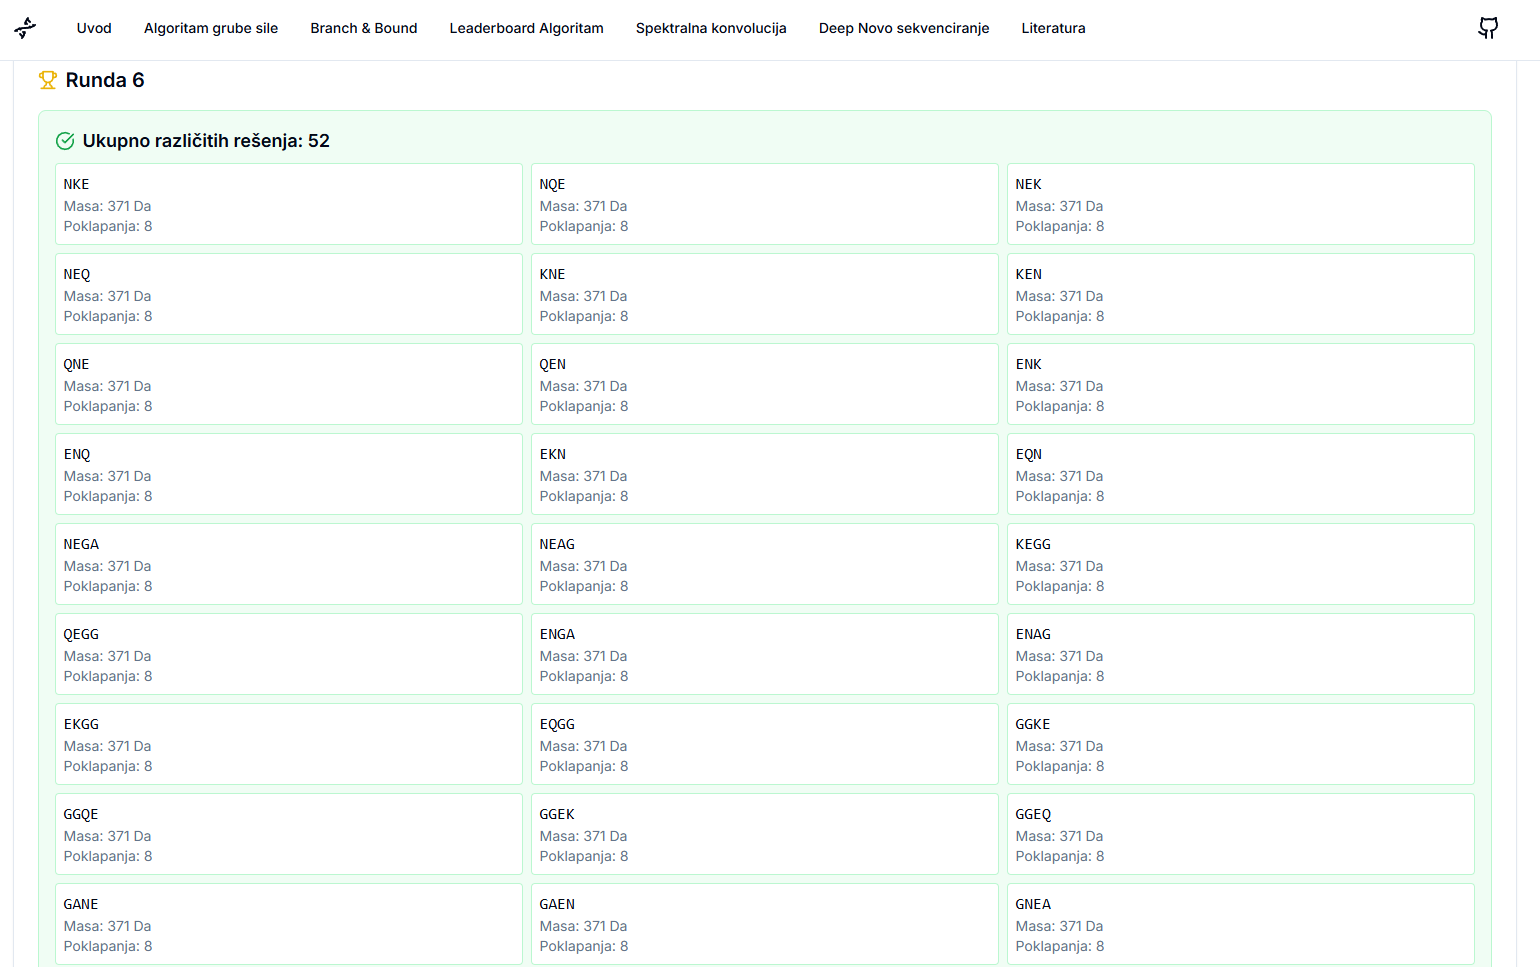
\includegraphics[width=1\textwidth]{images/leaderboard_3.png}
\caption{Poslednja runda i peptidi koji su rešenje za Leaderboard algoritam}
\label{fig:leaderboard_3}
\end{figure}

\subsection{Spektralna konvolucija}
Stranica za algoritam spektralne konvolucije, na slici \ref{fig:convolution_1}, sadrži objašnjenje ovog algoritma kao i kod u programskom jeziku \emph{Python} za implementaciju algoritma.
\begin{figure}[H]
\centering
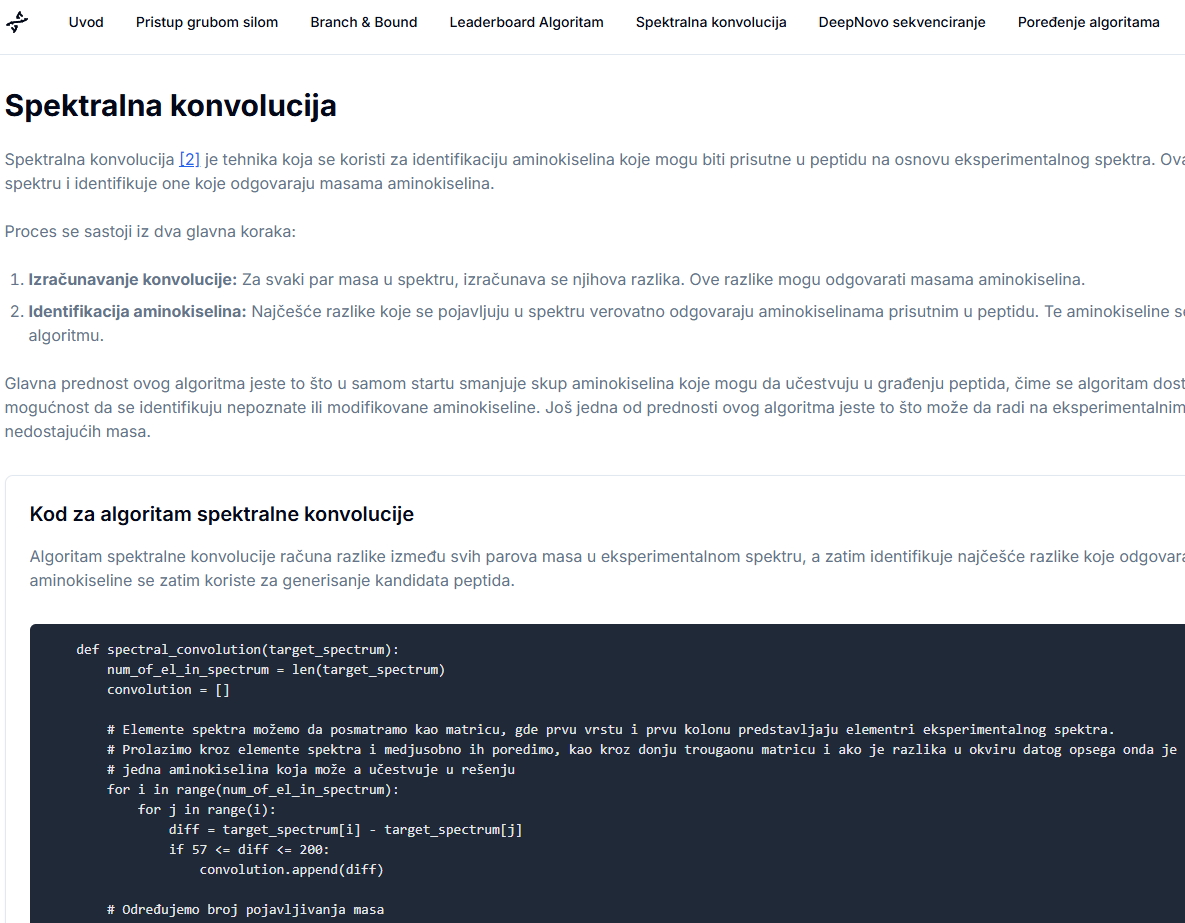
\includegraphics[width=1\textwidth]{images/convolution_1.png}
\caption{Stranica za algoritam spektralne konvolucije sa objašnjem istog}
\label{fig:convolution_1}
\end{figure}

Nakon objašnjenja i koda za algoritam može da se unese eksperimentalni spektar i može da se odabere da se vidi vizuelizacija ovog algoritma ili da se prikažu samo rešenja. Ovaj algoritam je veoma sličan \emph{Leaderboard} algoritmu, tako da je i vizuelizacija i elementi koji čine tu vizuelizaciju potpuno ista. Jedina razlika je što je ovaj algoritam na samom početku kreira matricu konvolucije, slika \ref{fig:convolution_2}, i uz pomoć matrice smanjuje broj aminokiselina koje mogu da učestvuju u izgradnji peptida, slika \ref{fig:convolution_3}. Postoje posebne kontrole za kontrolisanje animacije za izgradnju matrice konvolucije, kao i posebne kontrole za \emph{Leaderboard} deo ovog algoritma. Ove kontrole su slične onima iz prethodnih algoritama.

\begin{figure}[H]
\centering
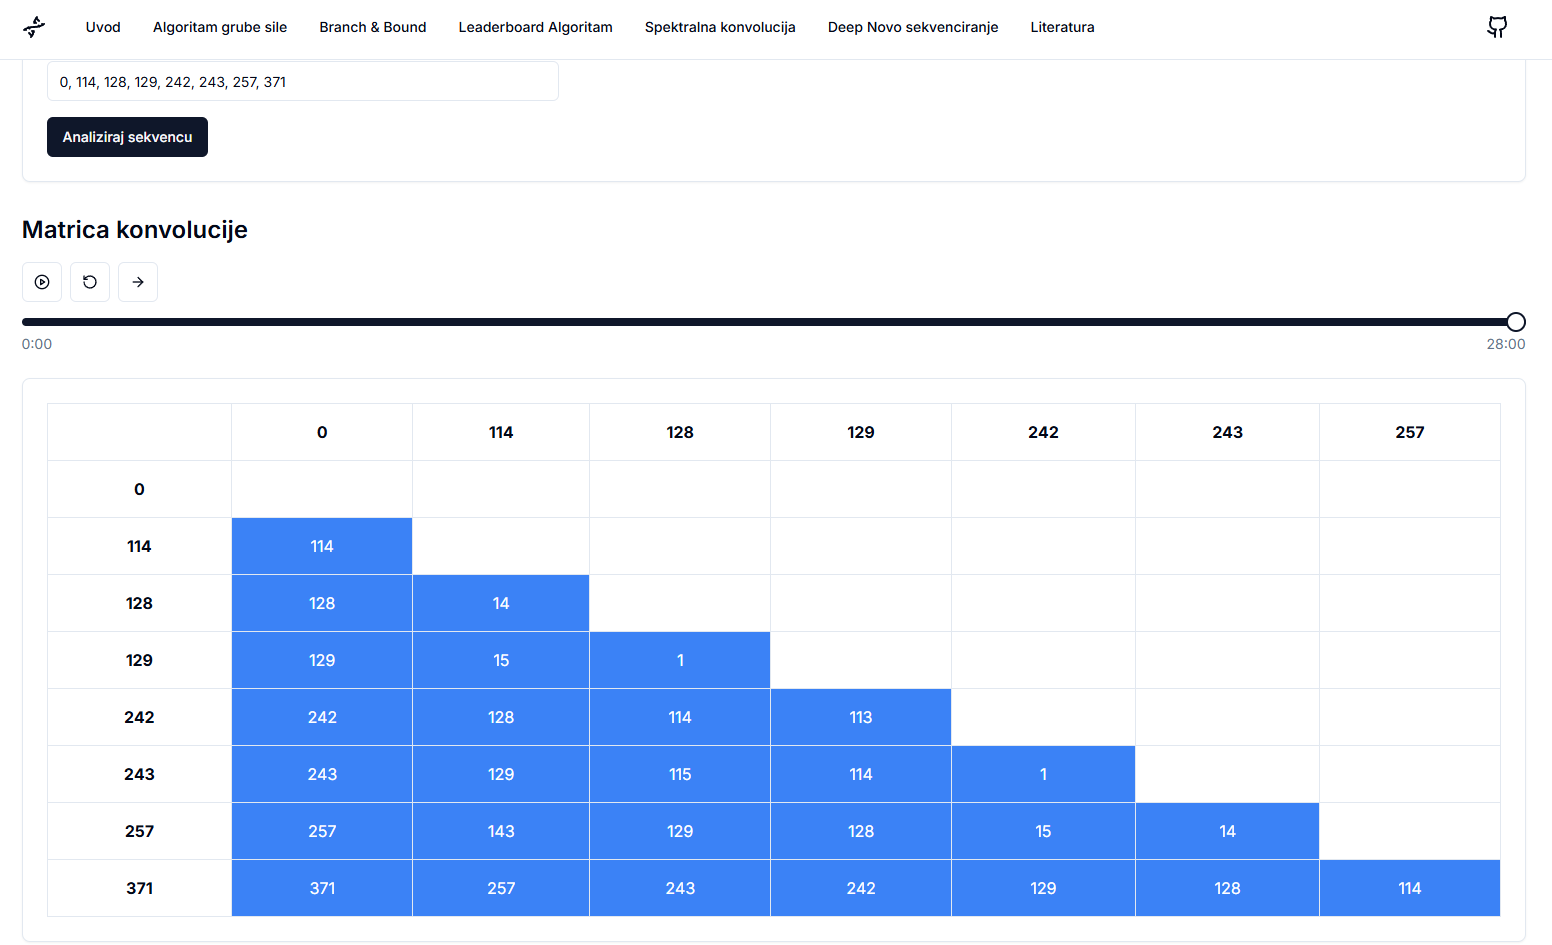
\includegraphics[width=1\textwidth]{images/convolution_2.png}
\caption{Matrica konvolucije u algoritmu spektralne konvolucije}
\label{fig:convolution_2}
\end{figure}

\begin{figure}[H]
\centering

\includegraphics[width=1\textwidth]{images/convolution_3.png}
\caption{Najčešće mase aminokiselina koje se pojavljuju u matrici konvolucije}
\label{fig:convolution_3}
\end{figure}

\subsection{\emph{DeepNovo}}
Stranica za \emph{DeepNovo} sekvenciranje, na slici \ref{fig:deepnovo_1}, sadrži \emph{tab}-ove koji pružaju uvid u detalje kao što su:
\begin{itemize}
    \item \textbf{Pozadina} - koji su trenutni problemi sekvenciranja
    \item \textbf{DeepNovo} - šta je DeepNovo i kako funkcioniše
    \item \textbf{Arhitektura} - koje komponente čine DeepNovo
    \item \textbf{Rezultati} - uspešnost primene DeepNovo metode
\end{itemize}

\begin{figure}[H]
\centering

\includegraphics[width=1\textwidth]{images/deepnovo_1.png}
\caption{Stranica za DeepNovo sekvenciranje}
\label{fig:deepnovo_1}
\end{figure}

\subsection{Poređenje algoritama}

Stranica za poređenje algoritama, na slici \ref{fig:comparison}, prikazuje vremena izvršavanja algoritama grube sile, \emph{Branch and Bound}, \emph{Leaderboard} i spektralne konvolucije. Dodatno, za svaki algoritam prikazuje i to da je pronašao rešenje i ako da koliko ih je. Na kraju će za svaki od algoritama biti prikazana i njegova rešenja. 

\begin{figure}[h]
\centering
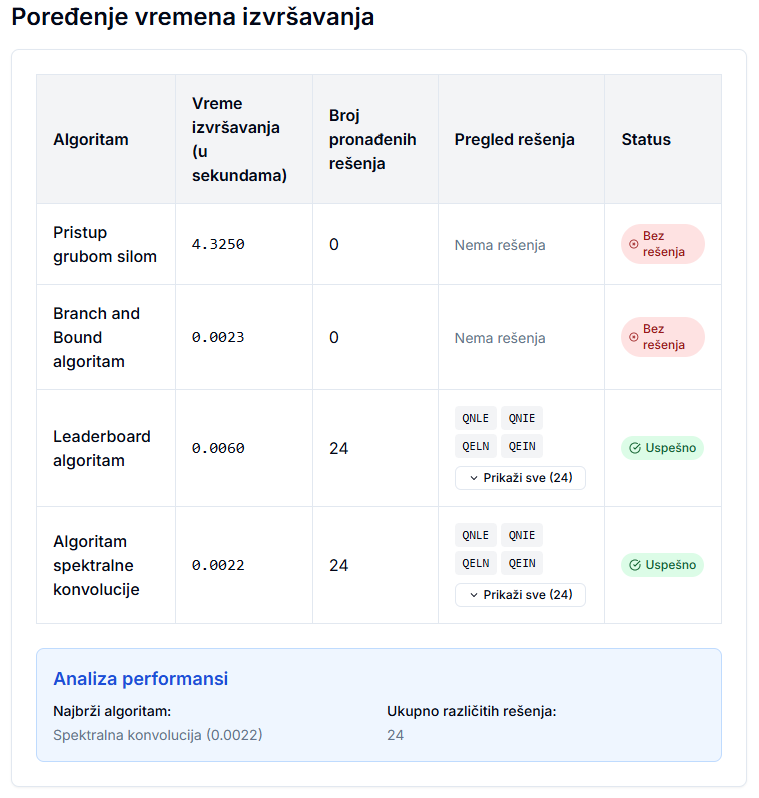
\includegraphics[width=1\textwidth]{images/comparison.png}
\caption{Poređenje brzine izvršavanja algoritama grube sile, \emph{Branch and Bound}, \emph{Leaderboard} i spektralne konvolucije}
\label{fig:comparison}
\end{figure}

\subsection{Nepostojeća stranica}

U slučaju da se unese pogrešan \emph{URL} za stranicu prikazaće se da ta stranica ne postoji i ponudi izbor postojćeih stranica, na slici \ref{fig:wrong_page} može da se to i vidi.

\begin{figure}[H]
\centering
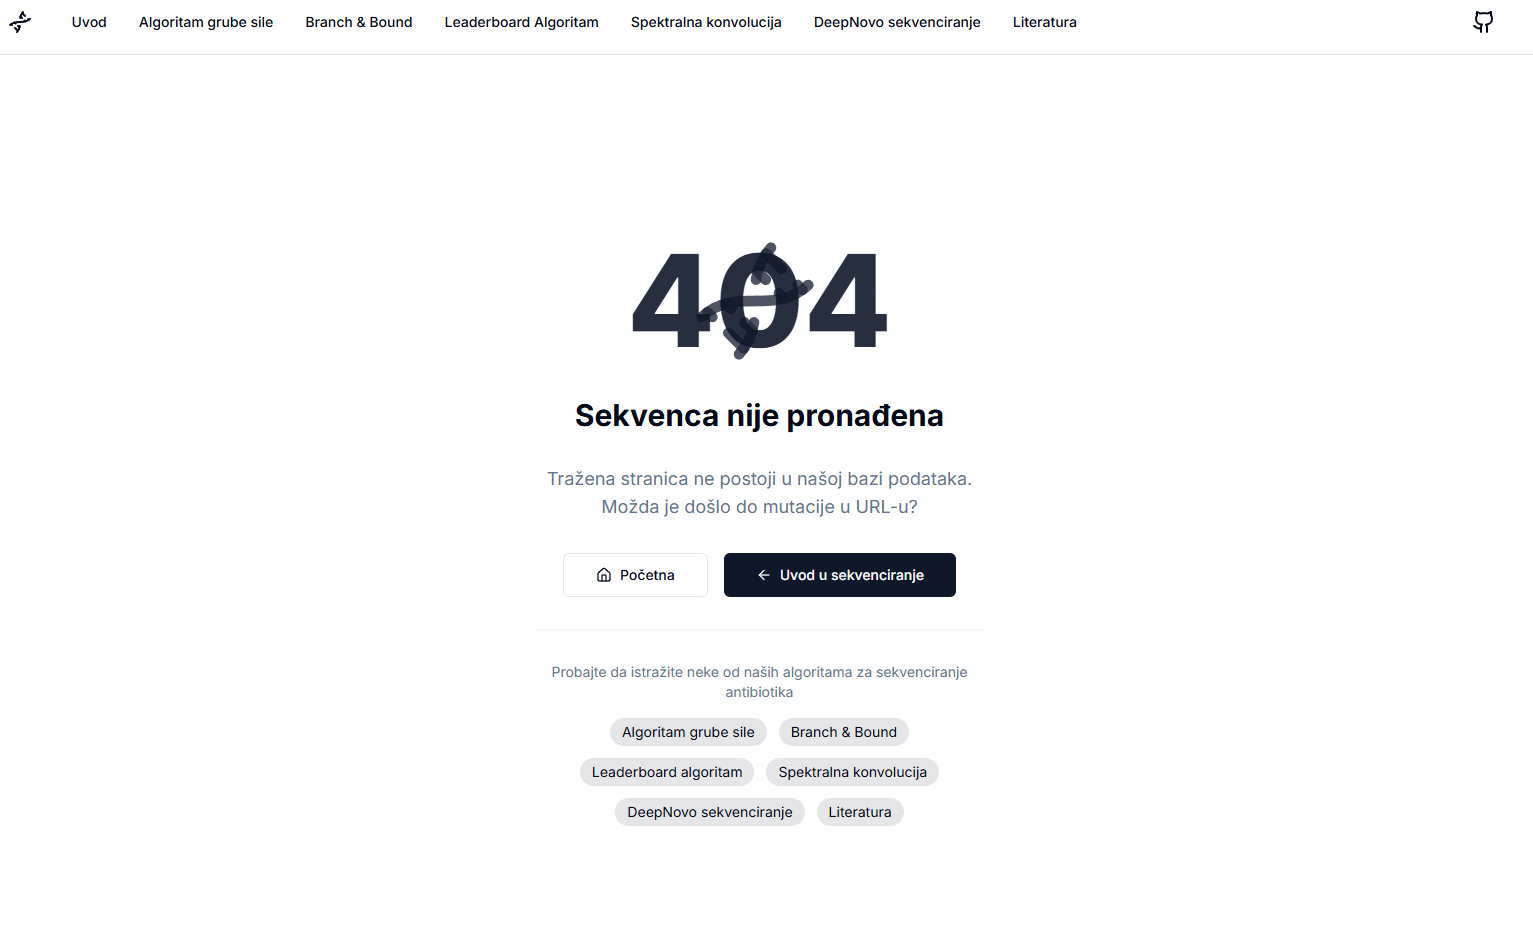
\includegraphics[height=0.5\textheight]{images/wrong_page.png}
\caption{Stranica koja se prikazuje u slučaju da je pogrešan \emph{URL} unet}
\label{fig:wrong_page}
\end{figure}

% ------------------------------------------------------------------------------
\chapter{Zaključak}
% ------------------------------------------------------------------------------

Razvijena elektronska platforma za sekvenciranje antibiotika predstavlja edukativni alat koji objedinjuje teorijske koncepte sa praktičnom implementacijom. Kroz interaktivne simulacije i vizuelizacije, platforma omogućava dubinsko razumevanje kompleksnih algoritama sekvenciranja.

Glavni doprinosi ovog rada uključuju:
\begin{itemize}
    \item Integraciju više algoritama za sekvenciranje u jedinstvenu platformu
    \item Vizuelizaciju koraka algoritama u realnom vremenu
    \item Kreiranje interaktivnog okruženja za učenje
    \item Poboljšanje dostupnosti bioinformatičkih alata studentima
\end{itemize}

Budući radovi mogu se usredsrediti na proširenje platforme sa dodatnim algoritmima, poboljšanje performansi postojećih implementacija i integraciju sa stvarnim eksperimentalnim podacima iz masene spektrometrije.

% ------------------------------------------------------------------------------
% Literatura
% ------------------------------------------------------------------------------
\literatura

% ==============================================================================
% Završni deo teze i prilozi
\backmatter
% ==============================================================================

% ------------------------------------------------------------------------------
% Biografija kandidata
\begin{biografija}
  \textbf{Miloš Milaković} rođen je 6. avgusta 1998. godine u Beogradu. Smer Informatika na Matematičkom fakultetu Univerziteta u Beogradu upisao je 2017. godine, a završio 2021. godine sa prosečnom ocenom 8.54. Nakon toga je upisao master studije na istom smeru. 
  Od septembra 2021. do marta 2024. godine je zaposlen na poziciji \emph{Software} developer u firmi \textbf{Endava}. Od marta 2024. godine do sada je zaposlen na poziciji \emph{Software} developer u firmi \textbf{LotusFlare}. Projekti na kojima je radio su uglavnom bili zasnovani na veb tehnologijama (\emph{Telco} industrija i \emph{FinTech} industrija), a osnovni programski jezik u kojem su projekti rađeni su \emph{Python}, \emph{Lua} i \emph{TypeScript}.
\end{biografija}
\end{document}